%PREAMBLE
\begin{comment}
%\documentclass[11pt]{article}
%\newcommand{\pablo}[1]{\textcolor{blue}{{\bf  #1}}}
\newcommand{\carlos}[1]{\textcolor{red}{{\bf  #1}}}
\newcommand{\fabio}[1]{\textcolor{purple}{{\bf  #1}}}
\newcommand{\susana}[1]{\textcolor{violet}{{\bf  #1}}}

% HEP names :: https://ctan.javinator9889.com/macros/latex/contrib/hepnames/hepnames.pdf

\DeclarePairedDelimiter\bra{\langle}{\rvert}
\DeclarePairedDelimiter\ket{\lvert}{\rangle}
\DeclarePairedDelimiterX\braket[2]{\langle}{\rangle}{#1 \delimsize\vert #2}

\newcommand*{\yt}{\ensuremath{y_{t}}\xspace}
\newcommand*{\tchannel}{\ensuremath{t\text{-channel}}\xspace}
\newcommand*{\schannel}{\ensuremath{s\text{-channel}}\xspace}
%\newcommand*{\lepT}{\ensuremath{\Pl_{\Pt}}\xspace}
%\newcommand*{\lepH}{\ensuremath{\Pl_{\PHiggs}}\xspace}

%\newcommand*{\muR}{\ensuremath{\mu_{\text{R}}}\xspace}
%\newcommand*{\muF}{\ensuremath{\mu_{\text{F}}}\xspace}

% Add external packages
\usepackage[italic]{hepnicenames}

%%%%%%%%%%%%%%%%%%%%%%%
%  From NA-HIGG-2020-02-INT1-defs.sty    %
%%%%%%%%%%%%%%%%%%%%%%%
% Basic tHq-related macros
%\newcommand*{\tHq}{\ensuremath{\Pqt{}\PH{}\Pq}\xspace}
%\newcommand*{\tHq}{\ensuremath{\Ptop \PHiggs \Pq}\xspace}
%\newcommand*{\tHq}{\Pqt{}\PH{}\Pq}
\newcommand*{\tHq}{\ensuremath{tHq}\xspace}
\newcommand*{\tH}{\ensuremath{\Pqt{}\PH{}}\xspace}
\newcommand*{\tHqsec}{\texorpdfstring{\Pqt{}\PH{}\Pq}{tHq}}
\newcommand*{\tHqML}{\ensuremath{\Pqt{}\PH{}\Pq\,(\text{ML})}\xspace}
\newcommand*{\tHqbb}{\ensuremath{\Pqt{}\PH{}\Pq\,(\bbbar)}\xspace}
\newcommand*{\tbarHq}{\Paqt{}\PH{}Pq}
\newcommand*{\tHbb}{\ensuremath{\tHq (\PH \to \bbbar)}\xspace}
\newcommand*{\tHtautau}{\ensuremath{\tHq (\PH \to \Pgt{}\Pgt)}\xspace}
\newcommand*{\dR}{\ensuremath{\Delta R}\xspace}
\newcommand*{\trexfitter}{TRExFitter\xspace}
\newcommand*{\thqloop}{\texttt{tHqLoop}\xspace}


\newcommand*{\MpT}{\ensuremath{\vec{p}_{\text{T}}^{\text{miss}}}\xspace}
\newcommand*{\mtw}{\ensuremath{m_{\text{T}}(\Pl,\MET)}}
\newcommand*{\mlb}{\ensuremath{m_{\Pl\Pqb}}}
\newcommand*{\mOSSF}{\ensuremath{m_{\text{OSSF}}}\xspace}

% Background processes
\newcommand*{\ttX}{\ensuremath{\Pqt{}\Paqt{}X}\xspace}
\newcommand*{\tX}{\ensuremath{\Pqt{}X}\xspace}

%\newcommand*{\ttX}{\Pqt{}\Paqt{}+X}
\newcommand*{\ttH}{\Pqt{}\Paqt{}\PH}
%\newcommand*{\ttH}{\ensuremath{\Pqt{}\Paqt{}\PH}\xspace}
\newcommand*{\ttZ}{\Pqt{}\Paqt{}\PZ}
\newcommand*{\ttV}{\ensuremath{\Pqt{}\Paqt{}V}\xspace}
\newcommand*{\ttW}{\Pqt{}\Paqt{}\PW}
\newcommand*{\ttWj}{\ensuremath{t\bar{t}W+j}\xspace}
\newcommand*{\tZq}{\Pqt{}\PZ{}\Pq}
\newcommand*{\tWZ}{\Pqt{}\PW{}\PZ}
\newcommand*{\tWH}{\Pqt{}\PW{}\PH}
\newcommand*{\tHW}{\Pqt{}\PW{}\PH}
\newcommand*{\tW}{\Pqt{}\PW}
\newcommand*{\Wt}{\Pqt{}\PW}
\newcommand*{\diboson}{diboson\xspace}
\newcommand*{\Diboson}{Diboson\xspace}
\newcommand*{\triboson}{triboson\xspace}
\newcommand*{\Triboson}{Triboson\xspace}
\newcommand*{\Vjets}{\ensuremath{V\text{+\,jets}}\xspace}

\newcommand*{\ttt}{\ensuremath{ttt}\xspace}
\newcommand*{\tttt}{\ensuremath{t\bar{t}t\bar{t}}\xspace}
\newcommand*{\ggH}{\ensuremath{ggH}\xspace}
\newcommand*{\qqH}{\ensuremath{qqH}\xspace}
\newcommand*{\WH}{\ensuremath{WH}\xspace}
\newcommand*{\ZH}{\ensuremath{ZH}\xspace}

% Fake leptons
\newcommand*{\elHF}{\ensuremath{e_{\text{HF}}}\xspace}
\newcommand*{\muHF}{\ensuremath{\mu_{\text{HF}}}\xspace}
\newcommand*{\elCo}{\ensuremath{e_{\text{conv}}}\xspace} 
\newcommand*{\kelHF}{\ensuremath{\mu(e_{\text{HF}})}\xspace}
\newcommand*{\kmuHF}{\ensuremath{\mu(\mu_{\text{HF}})}\xspace}
\newcommand*{\kelCo}{\ensuremath{\mu(e_{\text{conv}})}\xspace} 

% Signal regions
\newcommand*{\dileptau}{\ensuremath{2\Pl+1\tauhad}\xspace}
\newcommand*{\dilepOStau}{\ensuremath{2\Pl\,\text{OS}+1\tauhad}\xspace}
\newcommand*{\dilepSStau}{\ensuremath{2\Pl\,\text{SS}+1\tauhad}\xspace}

\newcommand*{\onelep}{\ensuremath{1\Pl}\xspace}
\newcommand*{\dilep}{\ensuremath{2\Pl}\xspace}
\newcommand*{\dilepOS}{\ensuremath{2\Pl\,\text{OS}}\xspace}
\newcommand*{\dilepSS}{\ensuremath{2\Pl\,\text{SS}}\xspace}
%\newcommand*{\SS}{\ensuremath{\text{SS}}\xspace}
%\newcommand*{\OS}{\ensuremath{\text{OS}}\xspace}

\newcommand*{\trilep}{\ensuremath{3\Pl}\xspace}
\newcommand*{\lepditau}{\ensuremath{1\Pl+2\tauhad}\xspace}




\newcommand*{\lumi}{\ensuremath{\mathcal{L}}\xspace}
\newcommand*{\lumiunits}{$\,$ cm$^{2} \,$s$^{-1}$\xspace}


%Other
\newcommand*{\CM}{\ensuremath{\sqrt{s}}\xspace}
 
\newcommand*{\Wtb}{\ensuremath{tWb}\xspace}
\newcommand*{\tWb}{\Wtb}
%\newcommand*{\tWb}{\ensuremath{tWb}\xspace}
\newcommand*{\pfour}{\ensuremath{\boldsymbol{\textrm{p}}}\xspace} 

\newcommand*{\tchan}{\ensuremath{t}-channel}
\newcommand*{\mtop}{\ensuremath{m_{\Ptop}}\xspace}
%\newcommand*{\mH}{\ensuremath{m_H}\xspace}
%\newcommand*{\HT}{\ensuremath{H_{\text{T}}}\xspace}

%\newcommand*{\PWplus}{\ensuremath{\PW^{+}}\xspace}
%\newcommand*{\PWminus}{\ensuremath{\PW^{-}}\xspace}
%\newcommand*{\Pgamma}{\ensuremath{\gamma}\xspace}

 \newcommand*{\greekphys}{\ensuremath{\varphi\upsilon\sigma\iota\kappa \eta}\xspace}
 \newcommand*{\greekatom}{\ensuremath{\alpha \tau o \mu o \nu}\xspace}
 \newcommand{\emu}{\ensuremath{\Pe/\Pmu}\xspace}

\newcommand*{\momentum}{\ensuremath{\overrightarrow{p}}\xspace} 
%\newcommand*{\CP}{\ensuremath{\mathcal{CP}}\xspace}
\newcommand*{\CP}{CP\xspace}

% Decays (Please, check latex/atlasprocess.sty and latex/atlasparticle.sty for more definitions!)
\newcommand{\bb}{\ensuremath{\Pqb\Paqp}\xspace}
\newcommand{\WW}{\ensuremath{\PW\PW^{*}}\xspace}
\newcommand{\ZZ}{\ensuremath{\PZ\PZ^{*}}\xspace}
\newcommand{\Higgsdecays}{\ensuremath{\PH \rightarrow b\bar{b}, \WW, \ZZ, \tau\tau}\xspace}
\newcommand{\Higgsdecayslep}{\ensuremath{\PH \rightarrow \WW, \ZZ, \tau\tau}\xspace}
\newcommand{\HWW}{\ensuremath{\PH \rightarrow \WW}\xspace}
\newcommand{\HZZ}{\ensuremath{\PH \rightarrow \ZZ}\xspace}

% reconstruction definitions
\newcommand{\pnutop}{\ensuremath{\vec{p^{\Pnu, \text{top}}}}\xspace}
\newcommand{\pnutopx}{\ensuremath{p^{\Pnu, \text{top}}_x}\xspace}
\newcommand{\pnutopy}{\ensuremath{p^{\Pnu, \text{top}}_y}\xspace}
\newcommand{\pnutopz}{\ensuremath{p_{z}(\Pnu_{\text{top}})}\xspace}
\newcommand{\pnutopT}{\ensuremath{\pT(\Pnu_{\text{top}})}\xspace}
\newcommand{\phinutop}{\ensuremath{\phi(\Pnu_{\text{top}})}\xspace}
\newcommand{\pltop}{\ensuremath{\vec{p^{\Plepton, \text{top}}}}\xspace}
\newcommand{\pltopx}{\ensuremath{p^{\Plepton, \text{top}}_x}\xspace}
\newcommand{\pltopy}{\ensuremath{p^{\Plepton, \text{top}}_y}\xspace}
\newcommand{\pltopz}{\ensuremath{p^{\Plepton, \text{top}}_z}\xspace}
\newcommand{\pltopT}{\ensuremath{\pT(\Plepton_{\text{top}})}\xspace}
\newcommand{\philtop}{\ensuremath{\phi(\ell_{\text{top}})}\xspace}
\newcommand{\phibtop}{\ensuremath{\phi(b_{\text{top}})}\xspace}
\newcommand{\tauvis}{\ensuremath{\Ptau_{\text{vis}}}\xspace}

\newcommand{\leptop}{\ensuremath{\Plepton^{\text{top}}}\xspace}
\newcommand{\lepH}{\ensuremath{{\Plepton^{\PH}}}\xspace}
\newcommand{\Hvismass}{\ensuremath{m_{\PH}^{\text{vis}}}\xspace}
\newcommand{\toprecomass}{\ensuremath{\mtop^{\text{reco}}}\xspace}
% \newcommand{\toprecomass}{\ensuremath{\Pqt_{\text{reco}}^{\text{m}}\xspace}}
% \newcommand{\Hvismass}{\ensuremath{\PH_{\text{vis}}^{\text{m}}\xspace}}
\newcommand{\MMC}{\texttt{MissingMassCalculator}\xspace}

% luminosity (2015)
\newcommand{\lumiFifteenRelUnc}{1.13} % in [%]
\newcommand{\lumitagFifteen}{{\small\texttt{OfLumi-13TeV-008}}}
%\newcommand{\lumiFifteenInPbNoUnits}{3219.56}
%\newcommand{\lumiFifteenInFbNoUnits}{3.2}
\newcommand{\lumiFifteenInPbNoUnits}{3244.54} % final luminosity recommendation for Run 2 analyses (https://twiki.cern.ch/twiki/bin/viewauth/Atlas/LuminosityForPhysics#2015_2018_13_TeV_proton_proton_f)
\newcommand{\lumiFifteenInFbNoUnits}{3.2}
%\newcommand{\dataperiodsFifteen}{D--J}
\newcommand{\dataperiodsFifteen}{D--H,J}
\newcommand{\firstdatarunFifteen}{276262}
\newcommand{\lastdatarunFifteen}{284484}
\newcommand{\datarunsFifteen}{\firstdatarunFifteen--\lastdatarunFifteen}
\newcommand{\dataeventsFifteen}{220.58M}

% luminosity (2016)
\newcommand{\lumiSixteenRelUnc}{0.89} % in [%]
\newcommand{\lumitagSixteen}{{\small\texttt{OfLumi-13TeV-009}}}
%\newcommand{\lumiSixteenInPbNoUnits}{32988.1}
%\newcommand{\lumiSixteenInFbNoUnits}{33.0}
% final luminosity recommendation for Run 2 analyses (https://twiki.cern.ch/twiki/bin/viewauth/Atlas/LuminosityForPhysics#2015_2018_13_TeV_proton_proton_f)
\newcommand{\lumiSixteenInPbNoUnits}{33402.2}
\newcommand{\lumiSixteenInFbNoUnits}{33.4}
%\newcommand{\dataperiodsSixteen}{A--L}
\newcommand{\dataperiodsSixteen}{A--G,I,K,L}
\newcommand{\firstdatarunSixteen}{297730}
\newcommand{\lastdatarunSixteen}{311481}
\newcommand{\datarunsSixteen}{\firstdatarunSixteen--\lastdatarunSixteen}
\newcommand{\dataeventsSixteen}{1057.84M}

% luminosity (2017)
\newcommand{\lumiSeventeenRelUnc}{1.13} % in [%]
\newcommand{\lumitagSeventeen}{{\small\texttt{OfLumi-13TeV-010}}}
%\newcommand{\lumiSeventeenInPbNoUnits}{44307.4}
%\newcommand{\lumiSeventeenInFbNoUnits}{44.3}
% final luminosity recommendation for Run 2 analyses (https://twiki.cern.ch/twiki/bin/viewauth/Atlas/LuminosityForPhysics#2015_2018_13_TeV_proton_proton_f)
\newcommand{\lumiSeventeenInPbNoUnits}{44630.6}
\newcommand{\lumiSeventeenInFbNoUnits}{44.6} 
%\newcommand{\dataperiodsSeventeen}{B--K}
\newcommand{\dataperiodsSeventeen}{B--F,H,I,K}
\newcommand{\firstdatarunSeventeen}{325713}
\newcommand{\lastdatarunSeventeen}{340453}
\newcommand{\datarunsSeventeen}{\firstdatarunSeventeen--\lastdatarunSeventeen}
%%%\newcommand{\datarunsSeventeen}{324320--341649}
\newcommand{\dataeventsSeventeen}{1340.80M}

% luminosity (2018)
\newcommand{\lumiEightteenRelUnc}{1.10} % in [%]
\newcommand{\lumitagEightteen}{{\small\texttt{OfLumi-13TeV-010}}}
%\newcommand{\lumiEightteenInPbNoUnits}{58450.1}
%\newcommand{\lumiEightteenInFbNoUnits}{58.5}
% final luminosity recommendation for Run 2 analyses (https://twiki.cern.ch/twiki/bin/viewauth/Atlas/LuminosityForPhysics#2015_2018_13_TeV_proton_proton_f)
\newcommand{\lumiEightteenInPbNoUnits}{58791.6}
\newcommand{\lumiEightteenInFbNoUnits}{58.8}
\newcommand{\lumiEightteenInPb}{\SI{\lumiEightteenInPbNoUnits}{\per\pb}}
\newcommand{\lumiEightteenInFb}{\SI{\lumiEightteenInFbNoUnits}{\per\fb}}
%\newcommand{\dataperiodsEightteen}{B--Q}
\newcommand{\dataperiodsEightteen}{B--D,F,I,K,L,M,O,Q}
\newcommand{\firstdataruEightteen}{348885}
\newcommand{\lastdatarunEightteen}{364292}
\newcommand{\datarunsEightteen}{\firstdataruEightteen--\lastdatarunEightteen}
%%%\newcommand{\datarunsEightteen}{348197--364292}
\newcommand{\dataeventsEightteen}{1716.77M}

% luminosity (2015+2016+2017)
%\newcommand{\lumiInPb}{80515.06~\invpb}
% \newcommand{\partlumi}{\SI{80.52}{\per\fb}}
%\newcommand{\datafirstyear}{2015}
%\newcommand{\datalastyear}{2017}

% luminosity (2015+2016+2017+2018)
%
% https://twiki.cern.ch/twiki/bin/viewauth/Atlas/LuminosityForPhysics#2015_2018_13_TeV_proton_proton_f
% final luminosity recommendation for Run 2 analyses (central value + uncertainty)
\newcommand{\lumiRelUnc}{0.83} % in [%]
\newcommand{\lumiInPbNoUnits}{140068.94} % in pb-1
\newcommand{\lumiInFbNoUnits}{140} % in fb-1
\newcommand{\lumiWithUnc}{\ensuremath{140.1 \pm 1.2}\,\si{\per\fb}} % in fb-1
%
% old recommendation
%\newcommand{\lumiRelUnc}{1.7} % in [%]
%\newcommand{\lumiInPbNoUnits}{138965.16} % in pb-1
%\newcommand{\lumiInFbNoUnits}{139} % in fb-1
%\newcommand{\lumiWithUnc}{\ensuremath{\lumiInFbNoUnits \pm 2.4}\,\si{\per\fb}} % in fb-1
\newcommand{\dataeventsAll}{4335.99M}
%
\newcommand{\lumiInPb}{\SI{\lumiInPbNoUnits}{\per\pb}}
%\newcommand{\lumi}{\SI{\lumiInFbNoUnits}{\per\fb}}
\newcommand{\datafirstyear}{2015}
\newcommand{\datalastyear}{2018}

% % tunes and PDF sets
\def\cteq{CTEQ6L1\xspace}
\def\ctten{CT10\xspace}
\def\cttennlo{CT10\,NLO\xspace}
\def\cttennnlo{CT10\,NNLO\xspace}
\def\ctfourteennlo{CT14\,NLO\xspace}
\def\ctfourteennnlo{CT14\,NNLO\xspace}
\def\nnpdfnnlo{NNPDF3.0\,NNLO\xspace}
\def\nnpdfnlofourflav{NNPDF3.0\,NLO\,nf4\xspace}
\def\nnpdfnlo{NNPDF3.0\,NLO\xspace}
\def\nnpdftwonlo{NNPDF2.3\,NLO\xspace}
\def\nnpdftwo{NNPDF2.3\,LO\xspace}
\def\nnpdftwofiveflav{NNPDF2.3\,5f\,FFN\xspace}
\def\mstw{MSTW2008\,NLO\xspace}
\def\a14{A14\xspace}
\def\auet{AUET2\xspace}
\def\aznlo{AZNLO\xspace}
\def\mmhtnnlo{MMHT2014\,NNLO\xspace}
\def\mmhtnlo{MMHT2014\,NLO\xspace}
\def\mmhtlo{MMHT2014\,LO\xspace}
\def\mstwnlo{MSTW2008\,68\%\,CL\,NLO \xspace}
\def\mstwnnloninety{MSTW2008\,90\%\,CL\,NNLO \xspace}
\def\ueee{UE-EE-5\xspace}




 
\endinput


%\begin{document}
asdf
%ENDPREAMBLE
\end{comment}




\chapter{Object reconstruction and identification}
%\pablo{Highlight the importance of alignment for the reconstruction}

%{\LARGE \textbf{}\\}
% The content of this section has to be general, i.e. it is valid for both the polarisation and the tHq analyses
%\tableofcontents
\label{chap:ObjectReconstruction}

\vspace*{0.1 cm} 
\hspace*{200pt} \\
\hspace*{175pt} \textit{El dos después del uno.} \\
%\hspace*{175pt} \textit{Primer el u i desrpés el dois.} \\
\hspace*{175pt} ---\textsc{Isabel Val}\\% \textit{} \\
\vspace*{2cm} 

%%%%%%%%%%%%%%%%%%%
%           Object reconstruction         %
%%%%%%%%%%%%%%%%%%%

The event reconstruction consists of the local pattern recognition (i.e. the
clustering and resolving of readout channels on the readout detector
elements), reconstruction of tracks, segments, vertices, cells and clusters in the
different sub-detectors, and finally the creation of high-level physical objects, such as
particles of different identification, jets including their flavour tag, or missing
energy estimation.

To reconstruct the physical objects, the information of all the subdetectors and systems of the ATLAS machine is employed.
A detailed description of all of these subsystems is presented in Section~\ref{chap:ATLAS}. 
After passing the trigger selection, the raw data are analysed to build the physics objects that constitute the
basic elements of any physical analysis. The process of  identifying and reconstructing these objects is described in this chapter.
Figure~\ref{fig:Chap2:ATLAS:ATLAS_Layers} illustrates how each particle interacts with the different layers of 
the ATLAS detector. 
The physical objects reconstructed and identified are the particle tracks and vertices (see Section~\ref{sec:Chap3:Reco:Tracking}), 
the leptons (see Section~\ref{sec:Chap3:Reco:Leptons}), the photons, jets and their flavour 
(see Section~\ref{sec:Chap3:Reco:jets}),
and the missing transverse momentum (see Section~\ref{sec:Chap3:Reco:MET}).
To avoid the reconstruction of the same energy deposits as multiple objects, overlap
removal criteria (see Section~\ref{sec:Chap3:Reco:OverlapRemoval}) are used.

%In order to have precise measurements it is necessary to have an excellent reconstruction of the particle in the
%final state. For measurements involving the top quark it is necessary to properly build the top decay products, i.e.
%electrons, muons jets \bjets and neutrinos (which are identified through the \MET)

\begin{figure}
	\centering
 	 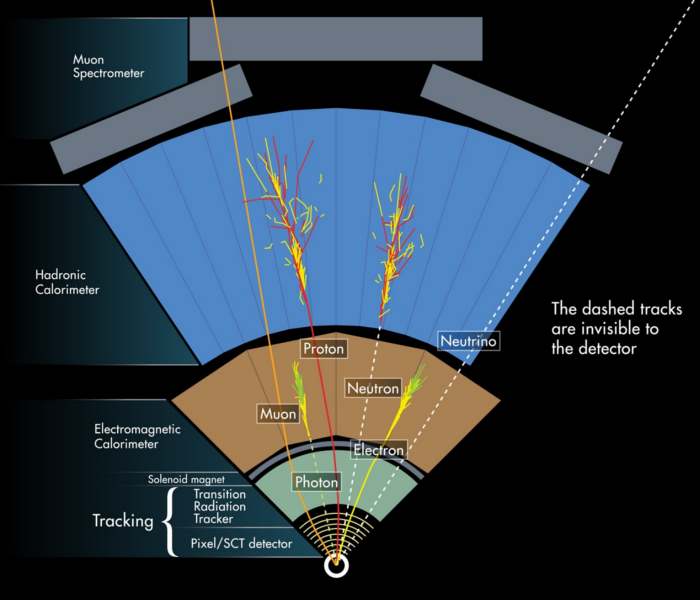
\includegraphics[width = 0.7\textwidth]{Chapter2/ATLAS_layers}
	 \caption{Fraction of the transversal plane of ATLAS. Each particle leaves a different signature in each layer~\cite{Pequenao:1505342}. 
	 By signature is meant the particular
	 distribution of energy deposition. This scheme is fundamental to understand the object reconstruction in this chapter. }
	\label{fig:Chap2:ATLAS:ATLAS_Layers}
\end{figure}

%%%%%%%%%%%%%%
%   Tracks and vertices     %
%%%%%%%%%%%%%%
\section{Tracks and vertices} % source: https://arxiv.org/pdf/1704.07983.pdf
\label{sec:Chap3:Reco:Tracking}
The detection and measurement of the momentum of the charged particles is an essential aspect of any large particle physics
experiment. Regardless of the medium through which a charged particle travels, it always leaves a trail
of ionised atoms and liberated electrons. By detecting this it is possible to reconstruct the trajectory of a charged
particle. 
%As introduced in Section~\ref{sec:Chap2:ID}, within the ATLAS detector, this is done by means of the silicon detectors in the ID. 

The trajectories followed by particles are referred to as ``tracks''. For charged particles, the tracks are reconstructed
using, mainly, the information of the ID (see Section~\ref{sec:Chap2:ID}) and, 
in the case of muons, the MS is also used (see Section~\ref{sec:Chap2:ATLAS:MS}).
 A charged particle passing through the ID will interact with its active sensors, the pixel detector and SCT
% (Figures~\ref{fig:Chap2:ATLAS:ID_PixelModule} and \ref{fig:Chap2:ATLAS:ID_SCT}, respectively)
 providing three-dimensional measurements as space-points.  
 While each two-dimensional hit in the pixel detector is directly translated into a space-point, for the SCT
 two one-dimensional hits are needed to reconstruct one space-point. %The TRT is used later
These space-points can be given by a single pixel activation or 
by several neighbouring pixels activated simultaneously (named cluster). 
Since the ID is immersed in a solenoidal magnetic field, the charged particles have their trajectories curved
by the Lorentz force, this allows to accurately calculate its $\pT$  using the sagitta method~\cite{ATLAS:2020ixw}.

The algorithms described in Section~\ref{sec:Chap2:ID_alignement}
are of fundamental importance to reconstruct high-quality tracks. 
This reconstruction is performed in two stages, the inside-out and the outside-in 
procedures~\cite{ATLAS:2017kyn}. 
The first is initiated from the centre of the ID and works outwards. 
This method is also used for the reconstruction of the primary vertex.
The inside-out algorithm starts by grouping the hits in the Pixel and SCT 
and merging them into clusters that are used to define the space-points. 
Secondly, the space-points are
combined in groups of three to form the track seeds. Then, a pattern-recognition
algorithm named Kalman filter~\cite{Fruhwirth:1987fm} is applied to build track
candidates from the seeds. This is accomplished by adding extra clusters from 
the remaining layers of the ID that are compatible with the estimated trajectory of the particles.
The Kalman filter provides several track candidates, so an ambiguity-solver algorithm
is applied to perform a stringent selection of the candidates. This compares the
individual track candidates by measurements of the track quality.
Finally,  the track candidates are then put through a high-resolution global $\chi^2$ fit,
which allows to further rejection of track candidates with a poor fit.

The inside-out method accounts for the majority of tracks reconstructed in the ATLAS detector but it 
is complemented by the outside-in, which 
starts in the TRT and works inwards. This method is used to find small-track segments
in the ID that were missed. 

The identification of the primary vertex is also of crucial importance
for the object reconstruction. This vertex identifies the IP
in which the hard-scattering process takes place. Therefore, the vertices are
defined by relating the origin of the track with individual points. The reconstruction
of the vertex is done in two complementary steps. First, the tracks are associated with
vertex candidates (vertex finding). Second, an iterative $\chi^2$ fit is used to determine the
best final three-dimensional location of the vertex. 

 


%\pablo{Highlight the importance of the alignment for the object definition and its reconstruction. Link this section with \ref{sec:Chap2:ID_alignement}}

\paragraph{Sagitta method}\mbox{}\\
%\subsection{Sagitta method}
\label{sec:Chap3:Reco:Sagitta}
The linear momentum (or just momentum) of a particle ($\overrightarrow{p}$) is one of the most important 
magnitudes in high-energy physics experiments because it provides information
about the energy of that particle. %In principle, using the tracks, it is not possible to determine the
%component of $\overrightarrow{p}$ in the direction of the beam. However, 
It is possible to determine the \pT of charged particles
by measuring the curvature caused by the magnetic field. In principle,
particles should have a straight trajectory but the magnetic field ($B$) curves its trajectory.
The \pT relates to the bending radius ($r$) by the Lorentz force:
\begin{align*}
	m\frac{v^2}{r} & = vqB\, , 
\end{align*}
from which one derives 
\begin{align*}
	\pT &=rqB \, ,
\end{align*}
where $q$ is the electrical charge of the particle and $v$ its speed. The $r$ is determined using
the arc length ($l$) and 
the sagitta ($s$), which is the distance from the centre of the trajectory arc the midpoint of its chord. Figure~\ref{fig:ChapReco:Sagitta} shows
in red the definition of sagitta. The radius is deduced by:
\begin{align*}
	r^{2}  = (l/2)^{2} + (r-s)^{2} \rightarrow r = \frac{(l/2)^2+s^2}{2s}\, .
\end{align*}
For high \pT particles $s \ll r$ and, hence, it is possible to approximate $r\sim\frac{l^2}{8s}$. 
The main uncertainty on \pT is the uncertainty on the sagitta and it can be
modelled with a Gaussian distribution.

\begin{figure}[h]
\centering
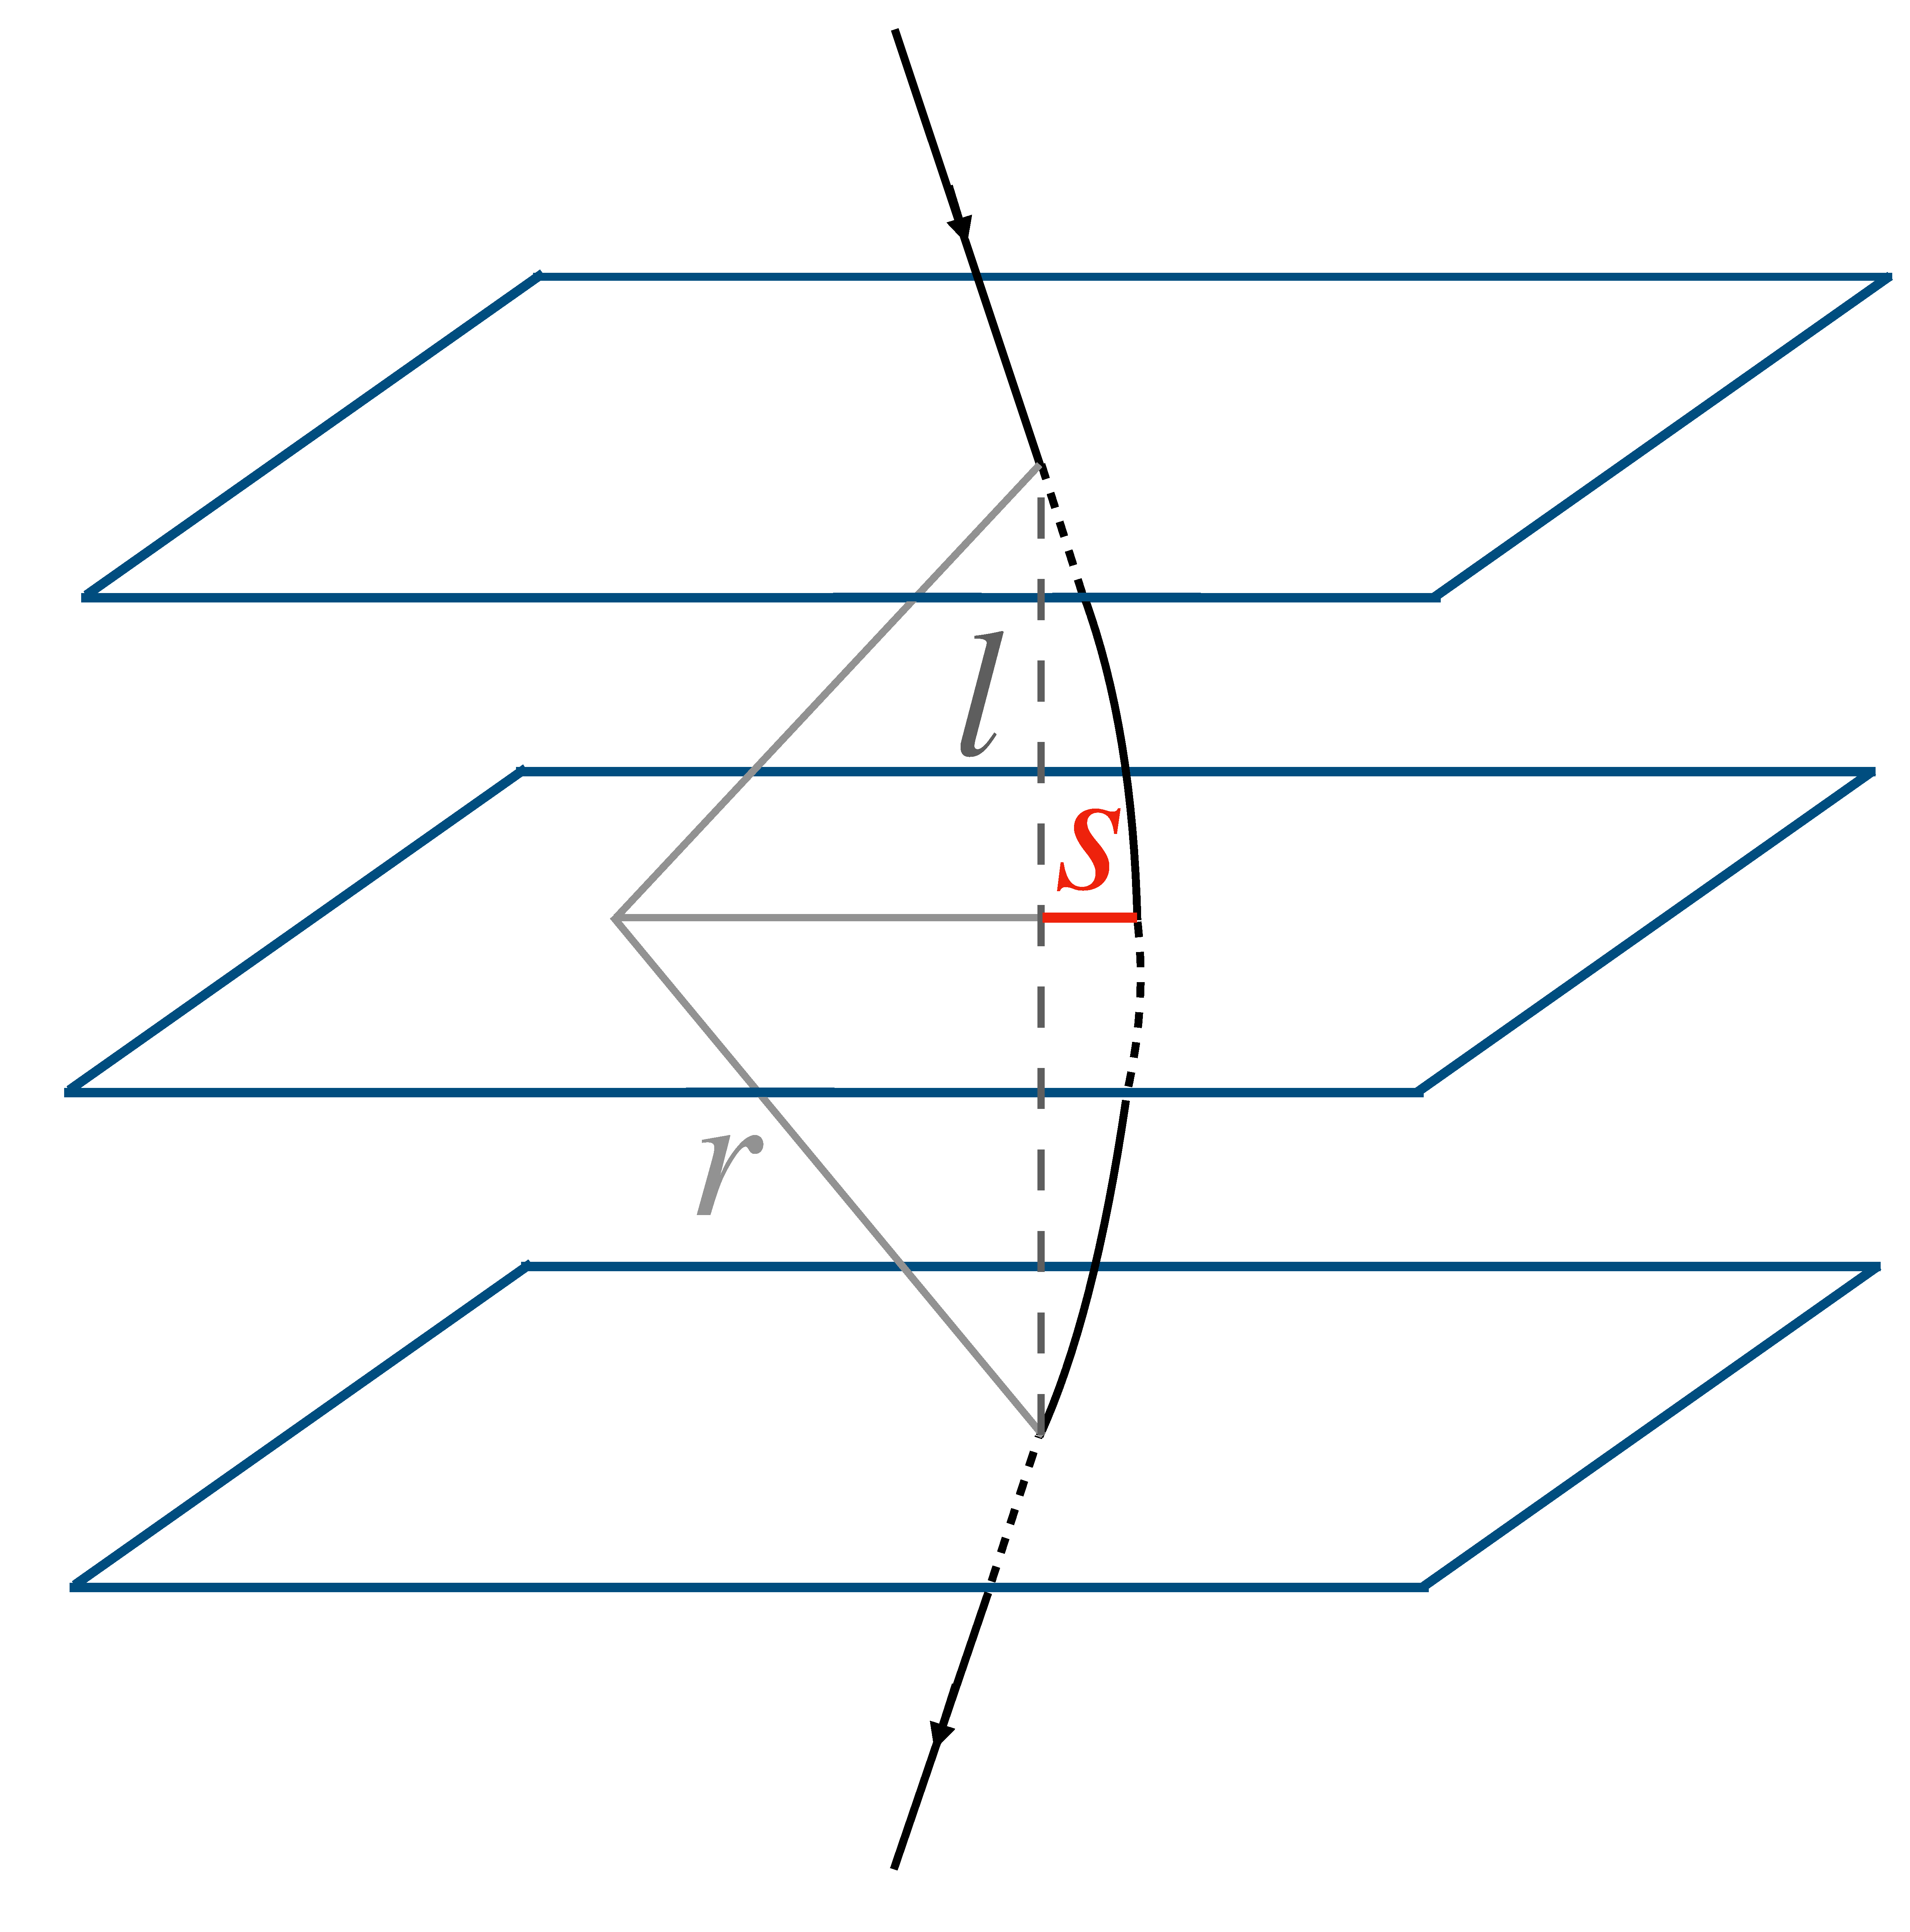
\includegraphics[width=0.5\textwidth]{Chapter3/Sagitta_method_byMe}
\caption{The arc represents the path of the particle. The layers of the tracker 
are drawn in blue. 
With the sagitta (red) and 
the arc length, the radius of curvature can be determined. The more energetic a
particle is, the larger is its bending radius.}
\label{fig:ChapReco:Sagitta}
\end{figure}



%%%%%%%%%
%   Letpons     %
%%%%%%%%%
\section{Charged leptons}
\label{sec:Chap3:Reco:Leptons}
The reconstruction of the charged leptons is a fundamental piece of many analyses, 
including the one developed in this thesis where the final state consists
of two light-flavoured-charged leptons (i.e. \emu) and one $\tau$-lepton  
decaying into hadrons. Therefore, the identification and reconstruction 
of the three leptons flavours is a key part of this thesis and is described
through the following subsections.


% Leptons :: Electron
\subsection{Electrons}
\label{sec:Chap3:Reco:ElectronsAndPhotons}
%For the reconstruction of electrons and photons, the algorithm first selects the top-clusters to consider when
%building these particles. It then 
% https://cds.cern.ch/record/2298955/files/ATL-PHYS-PUB-2017-022.pdf

The reconstruction of electrons\footnote{Note that the term electrons is used to 
collectively refer to electrons and positrons.} and photons is accomplished through 
the identification of energy deposits in the ECAL.
For the electrons, particle tracks recorded in the ID are required~\cite{ATLAS:2019qmc, ATLAS:2019jvq}.

%The only photons that are interesting for this analysis are the ones that 
%are misidentified as electrons. Besides that, no photon object is being reconstructied .

\paragraph{Electrons}\mbox{}\\
% Electron identification
In the analysis presented in this work, there are two final-state light-leptons 
that can be electrons. Therefore, accurate and efficient electron identification 
is crucial to measure our process of interest.
 Figure~\ref{fig:ChapReco:ElectronPath} presents 
a schematic representation of the ingredients composing the process 
of electron reconstruction and identification.
When an electron travels through the detector, it leaves traces in the ID
and energy deposits in the ECAL. The calorimeter signal activates the LVL1 trigger
and electron candidates are selected from an initial match between the ECAL energy
clusters and the ID tracks. %The energy clusters of the ECAL must have a value of $|\eta_{cluster}|$ less than 2.47, 
%excluding the transition region between the barrel and endcap calorimeters ($1.37 < |\eta_{cluster}| < 1.52$). 
The track associated with the electron must also pass on requirements  
on the longitudinal impact parameter 
$z_{0} \cdot \sin\theta < 0.5\,$mm and 
the transverse impact parameter $\frac{d_{0}}{\sigma(d_{0})} < 5$ where $\sigma(d_{0})$ is the uncertainty on $d_{0}$.
%Later, on Section~\ref{sec:ChaptH:EventSelection:PR}, this geometrical requirements for the reconstruction 
%are used to define the preselection region of the phase space. 

A typical electron candidate is expected to generate on average 12 hits in the inner tracker system, 
which includes one hit in the IBL layer, three hits in the silicon pixel layers, and 
eight hits in the SCT (4 double-sided silicon-strips layers).
Furthermore, approximately 35 straw hits are produced in the TRT system for an electron
of \pT larger than 500\;MeV. Finally, the electron moves to the ECAL, where the majority
of its energy is collected by the second layer.

The first step in the electron reconstruction is to build the clusters in the calorimeters.
To do so, the space in the ECAL is divided into small elements of dimension 
$\Delta \eta \times \Delta \phi =  0.025 \times 0.025$ that combine the subdetector layers. 
These elements are called towers. A presampler in the $|\eta|<1.8$ region also gathers the energy
and, along the first three layers of the ECAL, is used to determine the total energy per tower.
Clusters are seeded by individual towers with energy above 2.5$\,$GeV and are
searched for within the ECAL middle layer. Once the candidate clusters have been established,
the next step is to associate them with the tracks reconstructed in the ID using the tracking algorithms.

When multiple tracks can be linked to a specific EM calorimeter cluster, 
it is necessary to designate a primary electron track. This selection is performed 
through an algorithm that evaluates the $\eta$-$\phi$ distance between the extrapolated 
tracks and the cluster barycentre and considers the quantity of hits in the silicon 
detectors and the number of hits in the innermost silicon layers.
	
\begin{figure}
	\centering
 	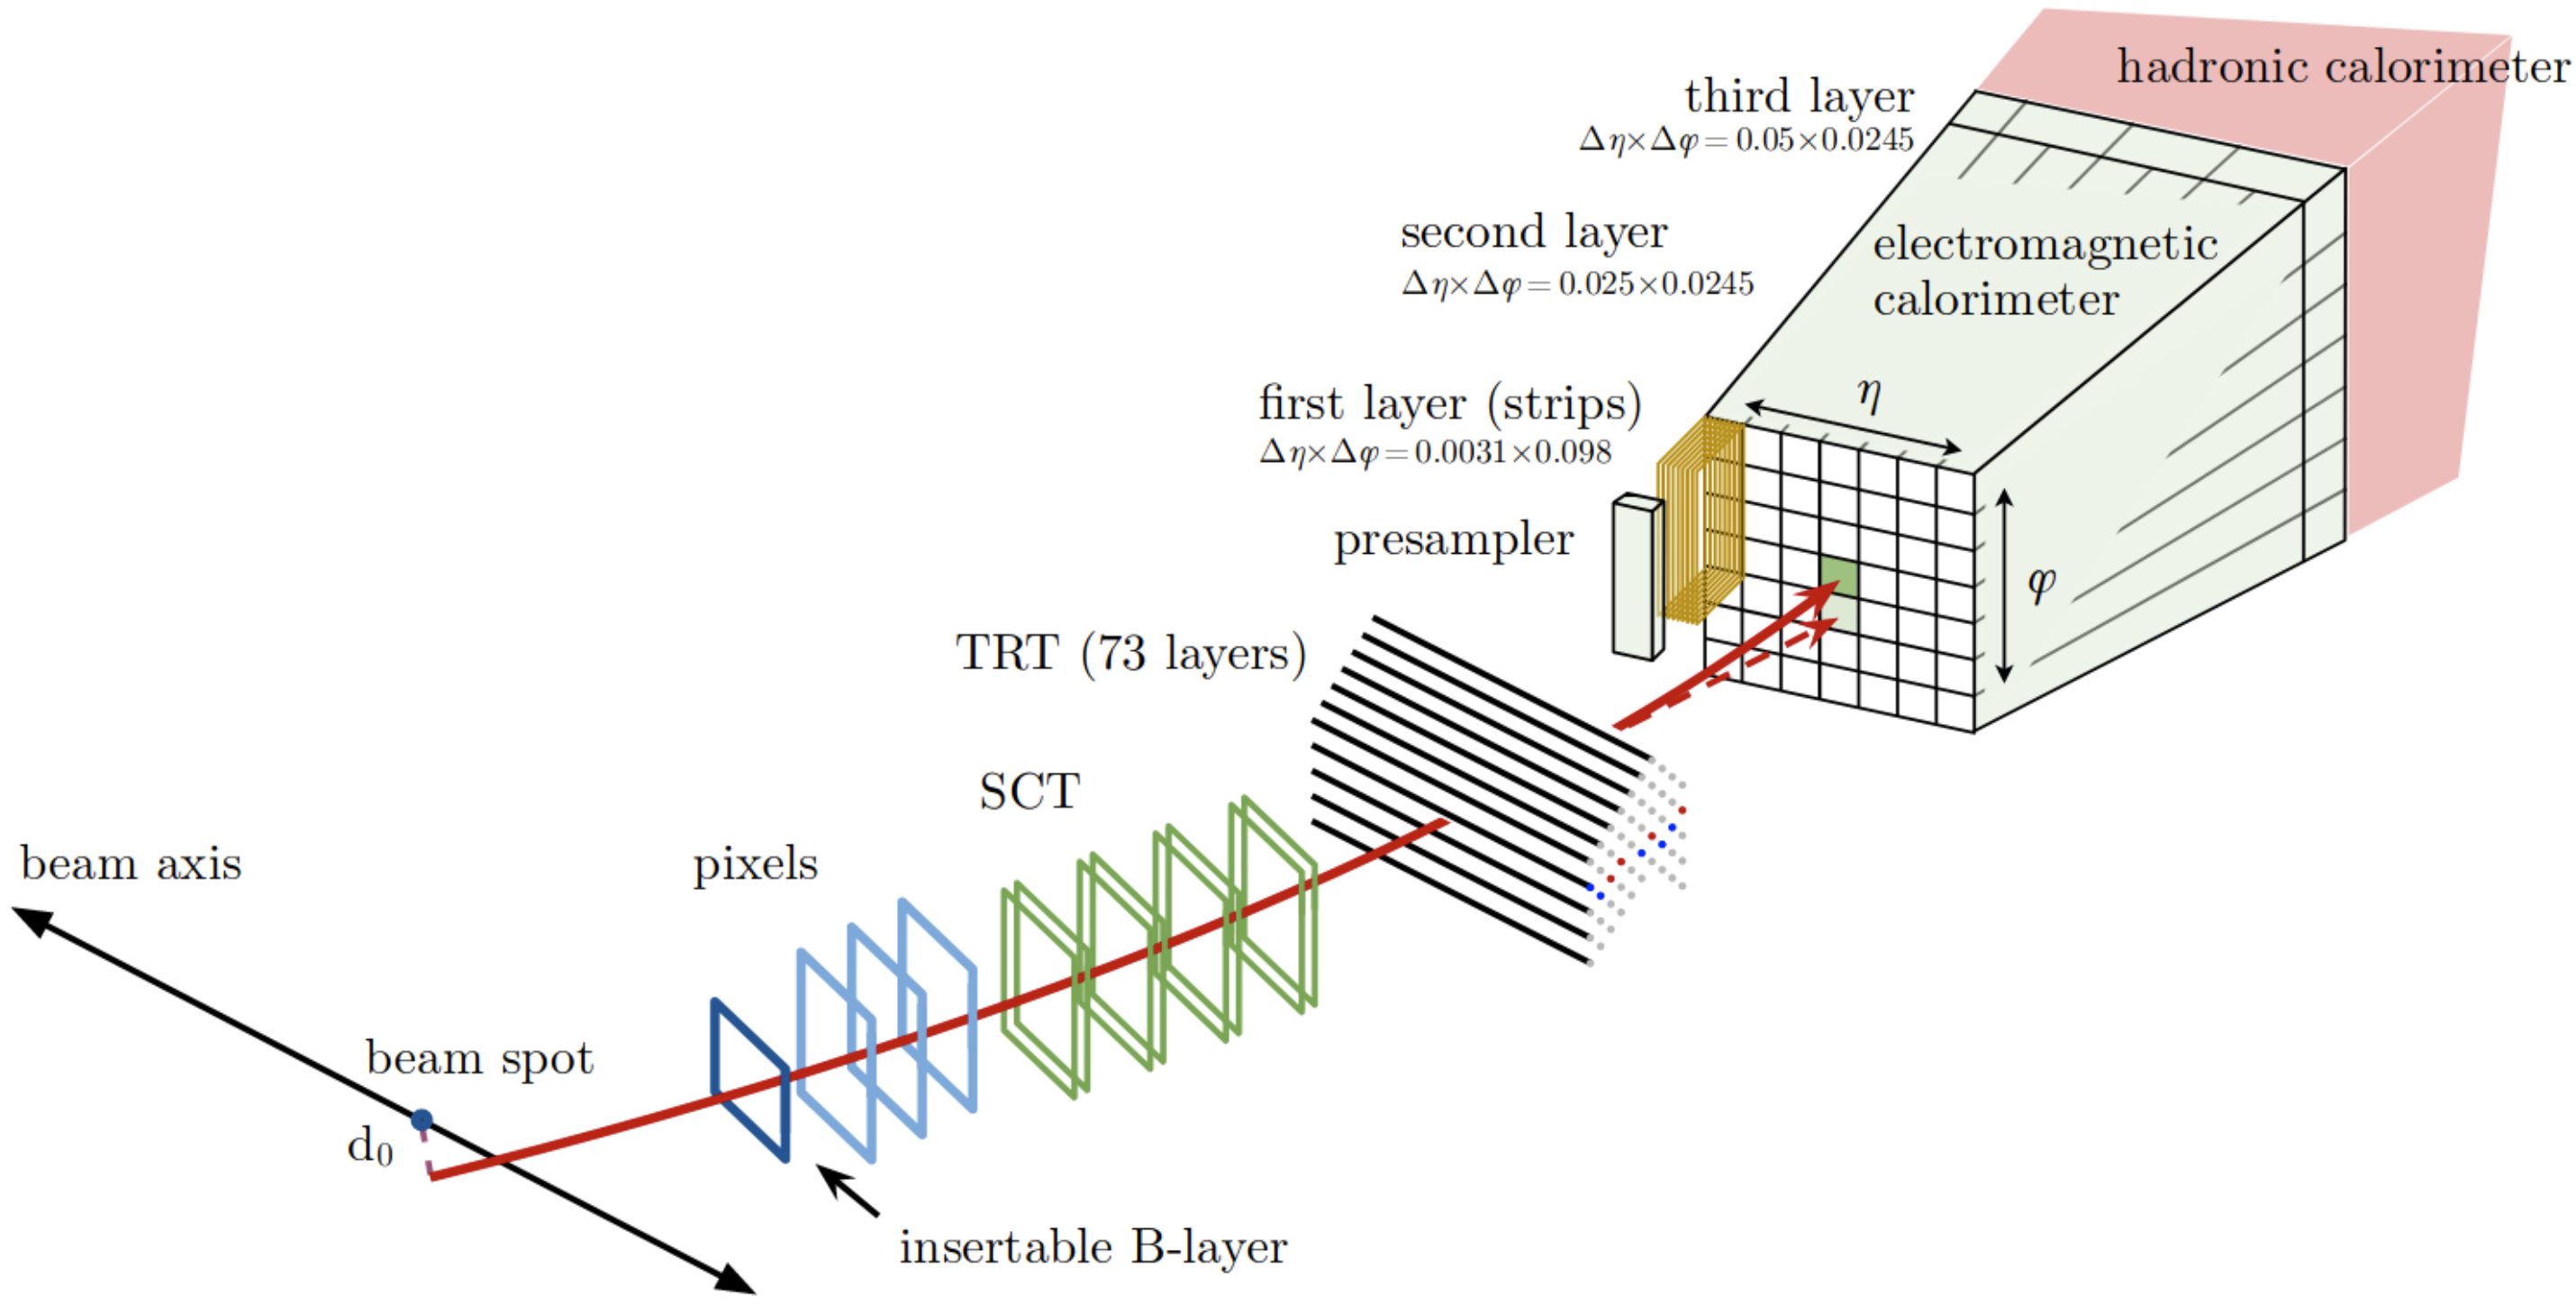
\includegraphics[width = \textwidth]{Chapter3/Objetct_Electron_Identification}
  	\caption{Trajectory of an electron through the detector. 
	The hypothetical path of the electron is represented by a solid red line, while the trajectory of a
	bremsstrahlung photon generated in the tracking system material is represented by a dashed red line.}
	 \label{fig:ChapReco:ElectronPath}
\end{figure}

%prompt and non-prompt electrons
Electrons may arise from either the primary hard-scattering event, such as the decay 
products of \PW or \PZ bosons (referred to as prompt electrons), or as the 
decay products of secondary particles with relatively long lifetimes, such as \Pbottom-hadrons 
(these are the so called non-prompt electrons). 
An example of non-prompt electron is presented in Figure~\ref{fig:ChapReco:NonPromptElectron}. 
The identification of prompt electrons is achieved through the use of a likelihood discriminant 
constructed from measurements taken in the ID and ECAL. The measured quantities are selected 
based on their effectiveness in distinguishing prompt-isolated electrons from energy deposits 
resulting from hadronic jets, from converted photons and non-prompt electrons. 
The discriminant considers the properties of the primary electron track, the lateral and longitudinal 
growth of the EM shower in the ECAL, and the spatial compatibility of the primary 
electron track with the cluster. 
Different operating points (working points) can be defined by setting fixed values for the likelihood discriminant.
These are \texttt{tight}, \texttt{medium} and \texttt{loose}. % (in ascending order of signal efficiency). 
The \texttt{tight} category is the most stringent, while the \texttt{loose} category is much more permissive in
terms of accepting something as an electron. In Section~\ref{sec:ChaptH:ObjectDefReco}, these categories are
used to define the trigger selection and the electron definition used in this analysis.

Regarding its charge, it is identified by the curvature of its track under the magnetic field. If the curve of the trajectory is not very pronounced, 
it can lead to misidentification of the charge. This phenomenon, known as charge flip, plays a role in the analysis described
in this thesis by being a relatively relevant source of background (as it is later presented in Table~\ref{tab:ChaptH:BkgEst:Origins}).
The charge flip can also emerge from bremsstrahlung radiation.


\begin{figure}
	\centering
 	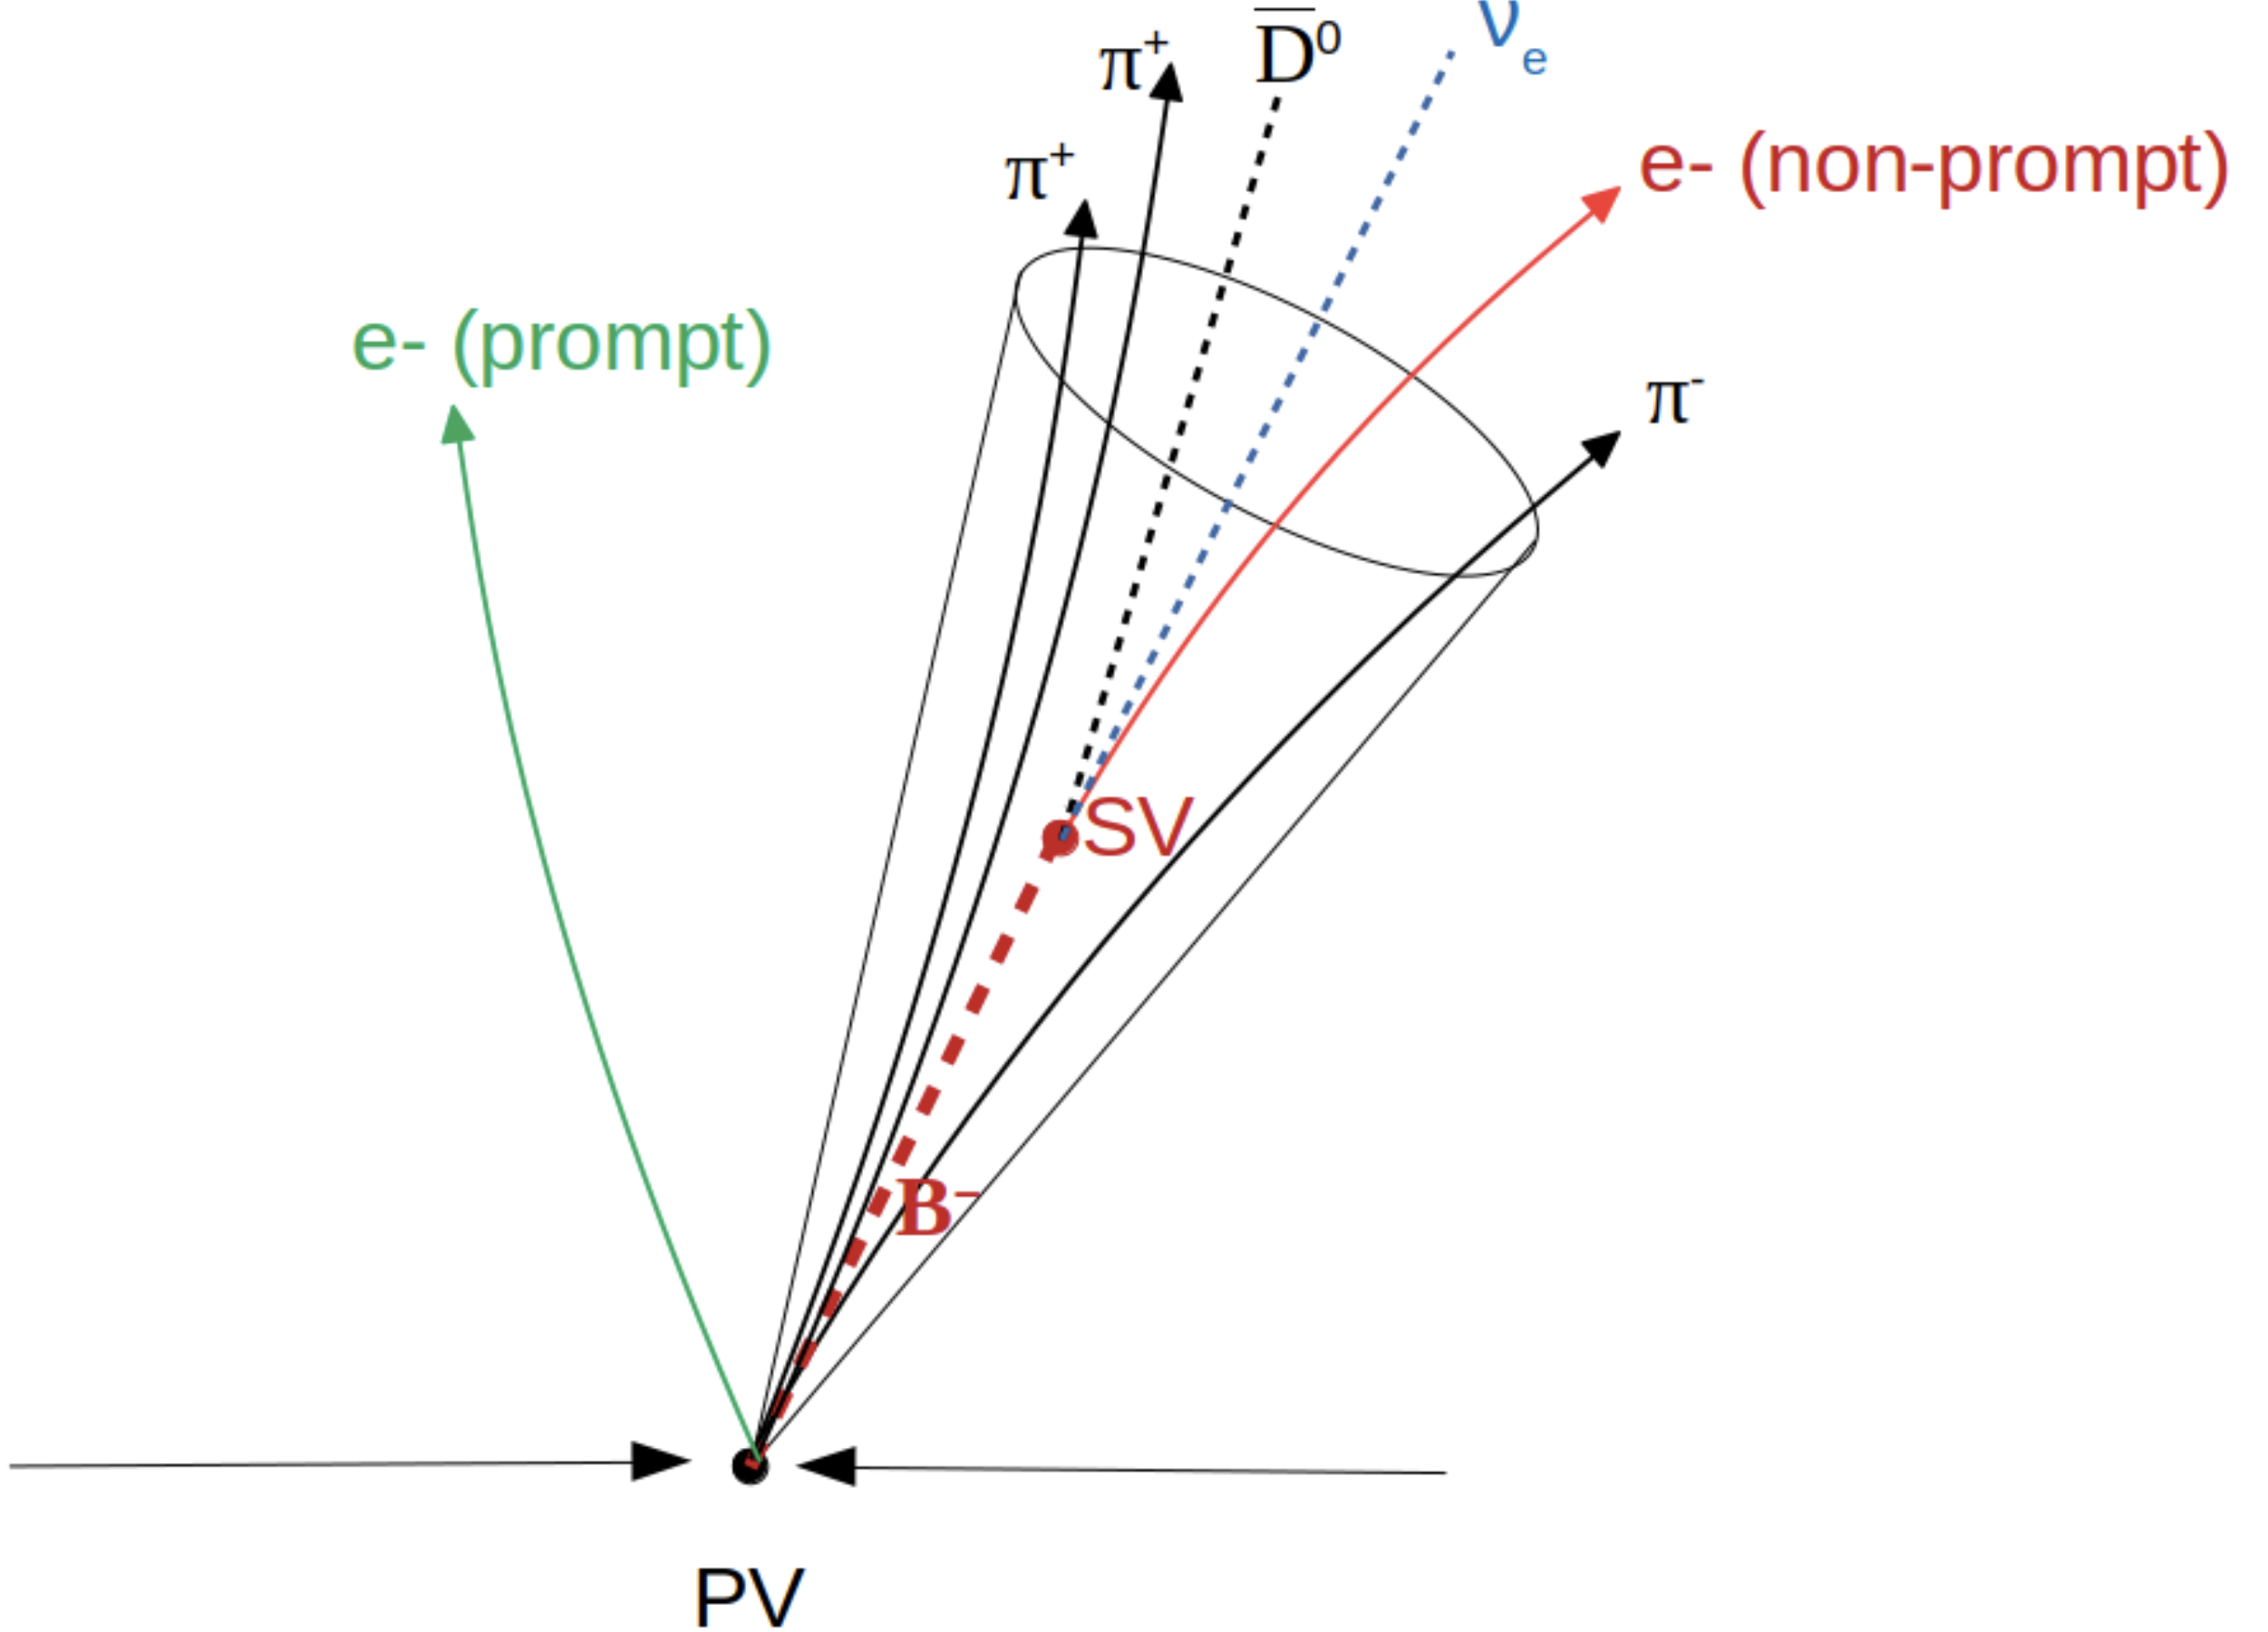
\includegraphics[width = 0.5\textwidth]{Chapter3/Objetct_fake_Ele_nonPromt}
  	\caption{A prompt electron depicted in green. 
	The cone symbolises a jet containing several hadrons.
	 The dashed red line corresponds to a \Pbottom-hadron (\PBminus),
	which decays into a \Pcharm-hadron (\APDzero), a neutrino (blue), and a non-prompt electron (red).
	The non-promt electron is originated from the secondary vertex while the prompt from the primary vertex.}
	 \label{fig:ChapReco:NonPromptElectron}
\end{figure}

Additionally, to differentiate the prompt electrons in signal processes from the background misidentifications,
isolation requirements are applied to the tracks and the calorimeter clusters. These are described in Reference~\cite{PERF-2017-01}.
% https://arxiv.org/pdf/1902.04655.pdf


%Calibration of electrons
The estimation of electron energy is derived from energy deposits in the ECAL and is 
subsequently refined through a series of calibrations to mitigate residual discrepancies 
between data and simulation~\cite{ATLAS:2014bzw}.
This calibration process includes the inter-calibration of the multiple calorimeter layers, 
corrections for energy shifts caused by pile-up, corrections that improve the uniformity 
of the energy response and changes to the overall energy scale.
Each correction is applied to the data to enhance accuracy.
Additionally, a correction to account for the difference in energy resolution between 
data and simulation is also applied to the simulated samples. 
The different uncertainties associated with this calibration stage are considered in the ATLAS analyses.

Finally, the electron-identification efficiency is determined for both real and simulated data using a
data-driven technique known as the tag-and-probe method~\cite{ATLAS:2011len}. The tag-and-probe is employed with  
the $\PZ \rightarrow \Pelectron \APelectron$ 
and $\PJpsi \rightarrow \Pelectron \APelectron$ decay modes. 
The tag-and-probe method relies on the preparation of an unbiased sample of physics objects, the \textit{probe} 
objects, which are used to calculate efficiencies and resolutions. The data sample is selected by means of an independent
\textit{tag} object~\cite{Straessner:1354502}.


% Photons
\paragraph{Photons}\mbox{}\\
The process of photon reconstruction closely mirrors that of electron reconstruction, 
with the primary distinction being the absence of tracks in the tracker, 
unless a photon undergoes conversion into an electron-positron pair,
in which case the corresponding tracks must be retrieved.

The identification working points are established with the ECAL information.
The distinction between prompt photons and background photons is achieved 
by applying selections based on quantities that characterise the shape and 
properties of the corresponding EM shower, as well as by 
implementing isolation criteria for the photon candidate.

% Leptons ::  Muon 
\subsection{Muons}
\label{sec:Chap3:Reco:Mu}
Muons can pass through every component of the ATLAS detector without being fully absorbed 
in the ECAL.
Therefore, the reconstruction of muon candidates within the ATLAS experiment involves a combination of 
information from the ID, the MS, and the calorimeters~\cite{ATLAS:2016lqx}. Muon candidates with $|\eta|<2.5$ are 
considered for reconstruction~\cite{ATLAS:2020auj}. 
In the MS, track reconstruction is accomplished 
by grouping hits into local track segments using a Hough transform~\cite{ILLINGWORTH198887}.
These segments are then merged to form track candidates, and a fitting procedure is employed to 
determine the trajectory of the muon within the magnetic field. Depending on the subdetectors 
involved in the muon reconstruction process, different types of muons can be identified:
\begin{itemize}
	\item Combined muons: This type of muon is identified by matching MS tracks to ID 
	tracks and performing a combined track fit using the hits from both systems. The energy
	loss in the calorimeters is taken into account during the fitting process.
	This definition works only for muons within $|\eta| < 2.5$, i.e. the ID acceptance.

	\item Inside--out muons: An \textit{inside--out} algorithm is utilised to reconstruct this category
	of muons. It extrapolates ID tracks to the MS and searches for at least three aligned MS 
	hits, which are then used for a combined track fit.

	\item Muon-spectrometer extrapolated: These muons arise when a MS track cannot be
	matched to an ID track. These muons are reconstructed in a range $2.5 < |\eta| < 2.7$ where the ID does not cover.
	In such cases, the parameters of the MS track are extrapolated to 
	the beam pipe to define the reconstructed muon. This type of 
	muon object is also referred to as stand-alone muon.

	\item Segment-tagged muons: This group of muons is identified by extrapolating ID tracks 
	to the MS and searching for matching segments. A muon is considered segment tagged if 
	an ID track is successfully matched to at least one MS segment, and the muon parameters 
	are directly obtained from the ID track fit. This allows an increase in the acceptance of
	muons which have crossed only one layer of the MS chamber.

	\item Calorimeter-tagged muons: In this scenario, muons are identified by extrapolating ID 
	tracks through the calorimeters to search for energy deposits consistent with those of a 
	minimum-ionising particle, i.e. a particle whose mean energy loss rate through matter is 
	close to the minimum value. If a match is found, the muon is identified as 
	calorimeter-tagged, and its parameters are again obtained from the ID track fit.	
	This type of reconstructed muons recovers acceptance in the region where 
	the MS is only partially instrumented.
\end{itemize}

%Depending on the identification requirement all muon options are reconstructed and taken 
%into account, as long as they are not overlapping. If this is the case a priority is given to the higher 
%quality muons, which would appear higher in the above list.


Prompt muons are identified by applying specific requirements on the number of hits in the ID 
and the MS, track-fit properties, and variables that test the compatibility between measurements 
in the two systems. 
Similarly to the electrons, 
the identification of muons requires that $z_{0} \cdot \sin\theta < 0.5\,$mm and 
$\frac{d_{0}}{\sigma(d_{0})} < 3$. 
The stringency of these requirements leads to three primary working points:
\texttt{tight}, \texttt{medium} and \texttt{loose}. As for electrons, the \texttt{tight} muons must meet 
more stringent requirements than the \texttt{loose} muons. 
The segment-tagged and calorimeter-tagged muons are considered in the loosest definition.
Additionally, two working points are designed for extreme phase space regions: the high-$\pT$ 
working point, which ensures optimal momentum measurement for muons with $\pT > 100$~GeV, 
and the low-$\pT$ working point, which addresses muons less likely to be fully reconstructed as 
tracks in the MS due to their low momentum.

To distinguish prompt muons objects from the misidentificated muons, isolation criteria are applied.
By demanding that $\Delta R=0.2$ cone around the tracks in the ID and around the energy clusters  
in the calorimeters, the non-prompt muons can be rejected~\cite{ATLAS:2020auj}. 

Corrections have been made to the simulated muon momentum scale and resolution to address
the observed discrepancies between the experimental data and simulation.
These discrepancies are studied using $\PZ \rightarrow \Pmuon \APmuon$ 
and $\PJpsi \rightarrow \Pmuon \APmuon$ decays. After implementing the corrections, data and %~\cite{Michael:2011jsa}
simulation agree to the per mille level for the muon momentum scale and to the percent level for the 
muon momentum resolution. The uncertainties arising from these corrections are quantified and propagated to 
the different ATLAS analyses.



% Leptons :: Tau
\subsection{Hadronically decaying taus}
\label{sec:Chap3:Reco:Tau}
%The identification of \Ptau-leptons is crucial for many analyses carried at the LHC.
On the one hand, the leptonically-decaying \Ptau-leptons (\taulep) cannot be differentiated from prompt
electrons or muons because \Ptau-decay takes place within several milimiters of the IP, 
i.e., before reaching the detector. Therefore, the \taulep are not identified. 
On the other hand, identifying hadronically-decaying \Ptau-leptons (\tauhad), while possible, is a challenging task. In this
section the identification and reconstruction of \tauhad is described.

%https://cds.cern.ch/record/1609659/files/ATL-GEN-PROC-2013-002.pdf
The \Ptau-lepton, being the most massive known lepton, exhibits a lifetime of approximately 
$2.9 \times 10^{-13}\,$s~\cite{Belle:2013teo}, which corresponds to an averaged travelled 
distance of 87~\textmu m in vacuum (assuming a momentum similar to the \Ptau mass). 
It predominantly decays into final states 
consisting of hadrons, accounting for approximately 65\% of its total decay modes. 
When doing so, it produces a \Ptau-jet containing a small number of
charged and neutral hadrons as it is shown in Figure~\ref{fig:Chap3:tau_jet}.
The formation of jets is described in Section~\ref{sec:Chap3:Reco:jets}.

\begin{figure}[h]
	\centering
 	 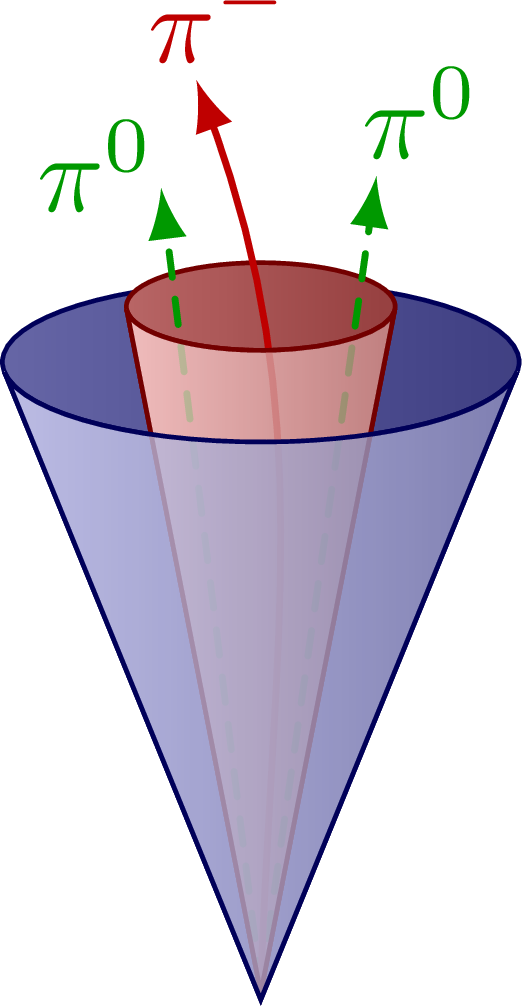
\includegraphics[width = 0.25\textwidth]{Chapter3/tau_jet_tkiz}
	 \hspace{0.05\textwidth}
	 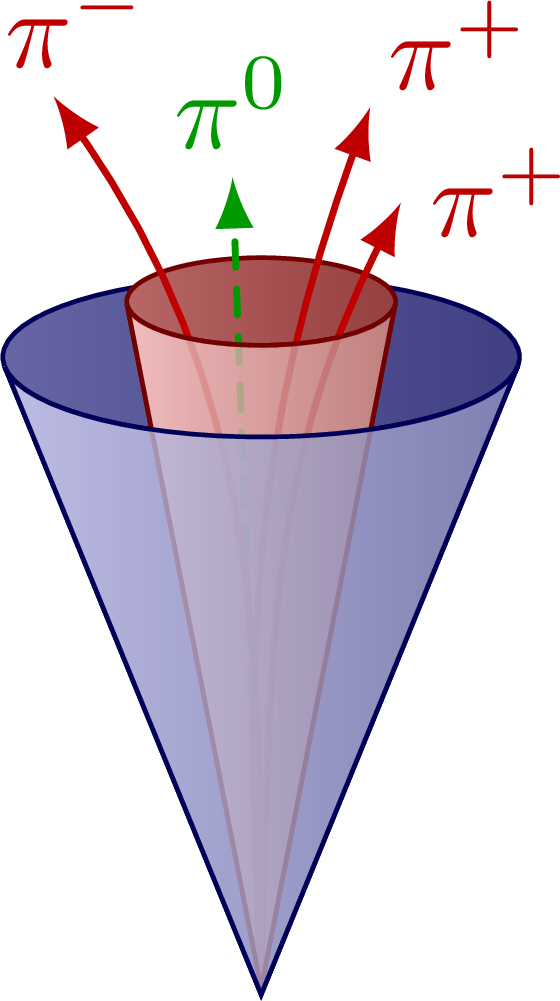
\includegraphics[width = 0.27\textwidth]{Chapter3/tau_jet_tkiz_moreProngs}
	 \hspace{0.05\textwidth}
	 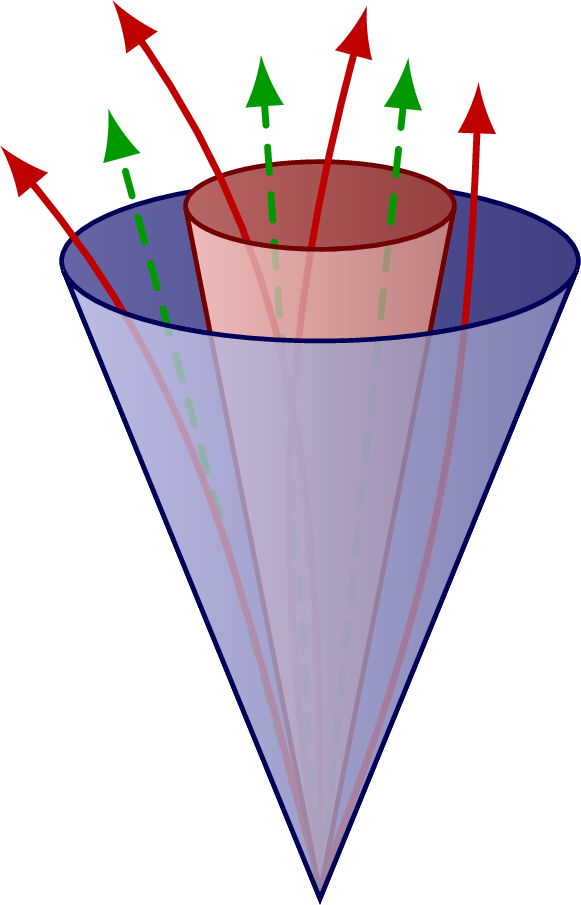
\includegraphics[width = 0.27\textwidth]{Chapter3/quark_initiated jet}
	 \caption{Isolation (blue) and signal cones (red) of hadronically-decayed taus in the left
	 and centre images. For comparison, a quark/gluon-initiated jet is presented on the right.
	 Note how the \Ptau-jets are more collimated.}
	\label{fig:Chap3:tau_jet}
\end{figure}

Hadronic decays of \Ptau-leptons exhibit distinct properties in terms of vertex displacement, track multiplicity, and kinematics. 
When the momentum of the \Ptau-lepton is large compared to its mass, a very collimated jet 
(the reconstruction of jets is described in Section~\ref{sec:Chap3:Reco:jets}) is
produced. %The reconstruction of jets is described with detail in Section~\ref{sec:Chap3:Reco:jets}.
For example, if the \Ptau-lepton carries a transverse momentum $\pT(\Ptau)>40\,$GeV, around
90\% of its energy is constrained within a cone of radius $\Delta R=0.2$. Other relevant property is that the \Ptau-lepton
decays exhibit low charged-track multiplicity of just one or three prongs\footnote{The term ``prong'' refers to 
the number of charged particles in the final state of the tau decay. As most detectors use a tracking chamber 
to identify charged particles, tau decays can be classified into those that provide a single track (1-prong) 
and those that provide three tracks (3-prong).}. Also, a relevant fraction of the EM energy 
deposition in the calorimeters is due to photons coming from the decay of neutral pions. %Quite often taus 
%are produced in pairs: in this case 42\% of final states will contain two \Ptau-jets~\cite{Bagliesi:2007qx}.
%In this specific analysis, this is the case when the Higgs boson decays to taus.
%Although, the top-quark system can decay into a single tau. 
In Table~\ref{tab:Chap3:Reco:Tau:DecayModes},
the main \Ptau-decay BR are shown. All these properties are exploited for the \tauhad identification.
 %The accurate identification and reconstruction of \Ptau-leptons decaying hadronically hold 
 %significant importance in numerous measurements and searches conducted at the LHC.
 
\begin{table}[h]
\centering
\begin{tabular}{l|c}
\toprule
Decay Mode & Fit Result (\%) \\
\midrule
$\mu^-   \bar{\nu}_{\mu}\nu_{\tau}$ & $17.3937 \pm 0.0384$ \\
$e^-   \bar{\nu}_{e}\nu_{\tau}$ & $17.8175 \pm 0.0399$ \\
$\pi^-   \nu_{\tau}$ & $10.8164 \pm 0.0512$ \\
%$K^-  \nu_{\tau}$ & $0.6964 \pm 0.0096$ \\
$\pi^-\pi^0   \nu_{\tau}$ & $25.4941 \pm 0.0893$ \\
%$K^-\pi^0   \nu_{\tau}$ & $0.4328 \pm 0.0148$ \\
$\pi^-2\pi^0   \nu_{\tau}$  & $9.2595 \pm 0.0964$ \\
%$K^-2\pi^0   \nu_{\tau}$ (ex. $K^0$) & $0.0647 \pm 0.0218$ \\
$\pi^-3\pi^0   \nu_{\tau}$ & $1.0429 \pm 0.0707$ \\
%$K^-3\pi^0   \nu_{\tau}$ (ex. $K^0, \eta$) & $0.0478 \pm 0.0212$ \\
%$h^-4\pi^0  \nu_{\tau}$ (ex. $K^0, \eta$) & $0.1118 \pm 0.0391$ \\
$\pi^- \pi^-\pi^+\nu_{\tau}$ & $8.9868 \pm 0.0513$\\
$\pi^- \pi^-\pi^+\pi^0\nu_{\tau}$ & $2.7404 \pm 0.0710$\\
$\pi^- \omega\nu_{\tau}$ & $1.9494 \pm 0.0645$ \\
\bottomrule
\end{tabular}
\caption{Most relevant \Ptau decay modes as listed by Reference~\cite{Workman:2022ynf}.}% reference~\cite{pdgTau}.}
% https://pdglive.lbl.gov/Particle.action?node=S035&init=0
\label{tab:Chap3:Reco:Tau:DecayModes}
\end{table}

%The \Ptau-leptons that decay to hadrons hold significant importance in the analysis under 
%consideration, as the \tauhad probably constitutes the most characteristic final-state object in the searches 
%for the \dileptau final state. Consequently, an accurate reconstruction of the \tauhad is crucial to 
%ensure the precise investigation of the underlying physical process. Notably, the primary cause of 
%background in this analysis stems from the misidentification of other objects (mainly gluon-initiated jets) as \tauhad, as it
%is shown in Section~\ref{sec:ChaptH:Bkg}.

The identification of \tauhad candidates use the calorimetric isolation and shape variables,
charged tracks isolation and other \Ptau-lepton characteristics suitable for tagging such as the impact parameter,
decay length and invariant mass.

%\begin{figure}
%	\centering
% 	 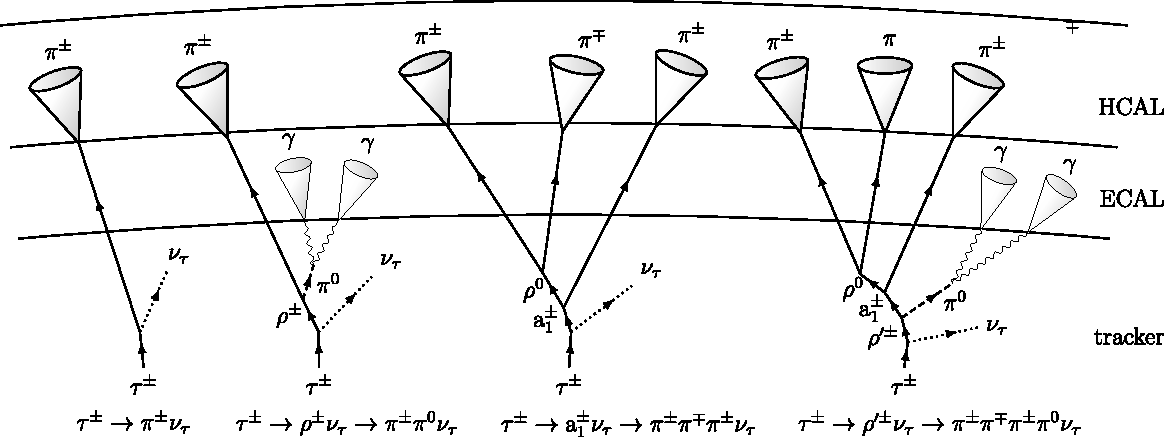
\includegraphics[width = \textwidth]{Chapter3/tau_ID}
%	 \caption{Hadronic tau reconstructed decays. The photons form the $\pi^0$ are detected in the
%	 ECAL and the $\pi^{\pm}$ in the HCAL. A  highly collimated quark or gluon jet can mimic these
%	 energy depoitis and be mistaken for any tau decay.}
%	\label{fig:Chap3:tau_tracks}
%\end{figure}

%\pablo{Incorporar también esto \url{https://cds.cern.ch/record/1045637/files/arXiv:0707.0928.pdf}. Tau Tagging at Atlas and CMS }


The \tauhad reconstruction involves the use of the anti-$k_t$ algorithm~\cite{Cacciari:2008gp}
with radius $R=0.4$. These \tauhad candidates originate from jet objects with $\ET >10\,$GeV and $|\eta|<2.5$. Subsequently,
tracks associated with the candidate are determined if they fall within the core region, defined by
a distance $\Delta R < 0.2$ from the jet barycentre. Additionally, tracks must satisfy specific 
quality criteria, including minimum \pT cut, hits in the silicon detector, and impact parameters.
Tracks within an isolation annulus ($0.2 < \Delta R < 0.4$) surrounding the barycentre are also 
employed to calculate identification variables but these tracks are not associated with the core region of the tau 
candidate~\cite{ATL-PHYS-PUB-2022-044, Leister:1609659}. The \tauhad candidates are categorised as 1-prong 
or multi-prong (primarily composed of three tracks). To correctly establish the charge and the number of charged 
decay products of a \tauhad , the tracks that are
associated with the \tauhad decay need to be correctly distinguished from the rest

To ensure optimal performance in high-pile-up scenarios, the Tau Jet Vertex Association~\cite{ATLAS:2014rzk}
algorithm is employed to determine the primary vertex of the \tauhad. This minimises the
influence of additional interactions, which could potentially lead to tau tracks failing to 
meet the $z_0$ impact parameter requirement~\cite{ATLAS:2012voa}.

The tau reconstruction alone provides limited rejection capabilities against 
various multi-jet backgrounds that can be challenging to differentiate from \tauhad. Several features of \tauhad, 
such as their narrow calorimeter clusters, isolation, and distinct 1- or 3-prong track signatures, 
can be exploited to discriminate between the jets and \tauhad.  During reconstruction, tracks 
and calorimeter clusters are employed to define several identification
variables that aid in distinguishing 
taus from quark- or gluon-initiated jets and other leptons. Variables that demonstrate substantial 
discriminatory power include those, characterising the shower shape in the calorimeter or tracks 
(e.g., energy fraction within $\Delta R < 0.1$ and average \pT-weighted track distance from the
tau axis) as well as those based on the track count.

To effectively suppress backgrounds arising from quark- or gluon-initiated processes, 
a set of multivariate algorithms collectively referred to as the tau identification have been 
developed by a dedicated ATLAS team. These algorithms use the aforementioned ID variables to
discriminate against jet backgrounds.
Two multivariate techniques, namely the projective likelihood method (LLH) and the method 
employing  boosted-decision trees (BDTs), are employed. The training of these algorithms involves the use of MC-event
samples of $\PZ \rightarrow \Ptau\Ptau$, $\PW \rightarrow \Ptau\Pnu_{\tau}$, and
$\PZ' \rightarrow \Ptau\Ptau$ for signal \tauhad, while jet-enriched data is utilised for 
background events.  The LLH and BDT are independently trained for 1-prong and multi-prong 
candidates. Each tau identification method establishes three thresholds based on the desired signal 
efficiency: \texttt{loose}, \texttt{medium} and \texttt{tight}. 
For 1-prong taus, the corresponding signal efficiencies obtained with the BDT+LLH method are
70\%, 60\%, and 40\%, respectively. While for multi-prong these are 65\%, 55\% and 35\%.
%source: https://cds.cern.ch/record/1609659/files/ATL-GEN-PROC-2013-002.pdf

Electrons and muons can also mimic the \tauhad signature. Similarly to the 
case of the jets misidentified as \tauhad, the electrons misidentified as \tauhad are discriminated by means of a 
BDT that is optimised using MC-event samples for $\PZ \rightarrow \Ptau\Ptau$ and 
$\PZ \rightarrow \Pe\Pe$ as background. The muons are misidentified with \tauhad 
when the muon track is associated with a sufficiently energetic calorimeter cluster.
To reduce the rate \Pmu identified as \tauhad, an algorithm requiring a certain criteria is used.

% Leptons :: Tau - Identification efficiency
\subsubsection{Tau identification efficiency}
To assess the effectiveness of the tau identification,
experimental data is directly used. The identification efficiency measurement
is achieved through a tag-and-probe method, which involves three distinct processes 
that considers decays to a single \tauhad:  $\PZ \rightarrow \taulep \tauhad$, 
$\PW \rightarrow \tauhad \nu_{\tau}$ and $\ttbar \rightarrow \tauhad + \text{jets}$.
 
The identification efficiency in data ($\epsilon_{\text{data}}$) is determined by comparing the
number of reconstructed \tauhad candidates (obtained from a fit to the number of tracks) before 
and after the tau identification is applied.  Similarly, the identification efficiency in simulated MC
events ($\epsilon_{\text{MC}}$) is also calculated. Scale factors, defined as the ratio of the 
identification efficiency in data to that in MC ($\epsilon_{\text{data}}/\epsilon_{\text{MC}}$), are 
then derived to quantify the performance of the tau identification. These scale factors are crucial 
in data analyses as they account for any discrepancies observed between the data and MC-event 
samples. In Table~\ref{tab:Chap3:Reco:Tau:eff}, the results obtained from the 
$\PZ \rightarrow \taulep \tauhad$ decay process are presented. These serve as the primary
 measurement due to their high precision, owing to the low associated backgrounds.
The results from the $\PW \rightarrow \tauhad \nu_{\tau}$ process are used as a cross-check, 
while the $\ttbar \rightarrow \tauhad + \text{jets}$ process provides a measurement for a higher
 kinematic regime, particularly for higher \pT values.

\begin{table}[h]
\centering
\begin{tabular}{l|c|c}
\toprule
       		& BDT                       				& LLH                 \\ \midrule
\texttt{loose}  	& $1.033 \pm 2.0\% \pm 1.0\%$ 	& $1.044 \pm 1.7\% \pm 1.0\%$ \\
\texttt{medium} 	& $0.979 \pm 2.1\% \pm 1.1\%$    	& $0.985 \pm 2.1\% \pm 1.1\%$ \\
\texttt{tight}  	& $0.907 \pm 2.6\% \pm 1.5\%$    	& $0.941 \pm 2.4\% \pm 1.5\%$ \\ \bottomrule
\end{tabular}
\caption{\tauhad identification efficiency measurements performed with $\PZ \rightarrow \taulep \tauhad$ decays~\cite{Leister:1609659}. 
Results presented as ``scale factor $\pm$ systematic uncertainty $\pm$ statistical uncertainty''.}
\label{tab:Chap3:Reco:Tau:eff}
\end{table}

%\pablo{Añadir en esta sección la información de este paper:
%\url{https://arxiv.org/pdf/2211.16178.pdf}. "Tools for estimating fake/non-prompt lepton
%backgrounds with the ATLAS detector at the LHC"}



%%%%%%%
%    Jets     %
%%%%%%%
\section{Jets}
\label{sec:Chap3:Reco:jets}
%At detectors for accelerator-based experiments, quarks and gluons are detected by the jets of hadronic particles that they produce
%in the detector soon after they are created.
When a quark or gluon is produced in high-energy processes, it cannot exist in isolation due to 
the colour confinement as it is stated in Section~\ref{sec:chap1:QCD}.
%The suppression of quarks is due to colour confinement as it is stated in Section~\ref{sec:chap1:QCD}.
An exception to this rule are the top quarks, whose lifetime is smaller than the hadronisation time by two orders of
magnitude and, hence, they are detected by their decay products. 
For the gluons and the rest of quarks, hadronisation showers %(Section~\ref{sec:Chap2:CALO:Shower}) 
take place and jet-clustering algorithms merge the clusters and tracks produced by these jets
to reconstruct them. There are two algorithms to reconstruct jets: the cone  %~\cite{Atkin:2015msa}
algorithms~\cite{UA1:1983hhd} and the sequential clustering algorithms~\cite{Catani:1993hr}. 

In the majority of ATLAS analyses, the sequential clustering ``anti-$k_t$'' algorithm 
is used~\cite{Catani:1993hr, CMS-PAS-JME-09-001, Cacciari:2008gp} to analyse the data
from hadronic collisions. To model a jet as a cone, this algorithm uses a specific choice of radius parameter 
($R$) defining the radial size of the jet. 
The distance between all pairs of objects $i$ and $j$ ($d_{ij}$) and the distance between the 
objects and beam pipe ($d_{iB}$) are used in: 
\begin{align*}
	d_{ij} 	&= \text{min}(p^{2f}_{\text{T}i}, p_{\text{T}j^{2f}}) \frac{\Delta R_{ij}^{2}}{R^{2}}\, , \\ \label{eq:chap3:antikt_1}
	d_{iB} 	&= p^{2f}_{\text{T}i}\, ,
\end{align*}
where
\begin{equation*}
	\Delta R_{ij}^{2} = (y_{i} - y_{j})^{2} - (\phi_{i} - \phi_{j})^2
\end{equation*}
and $p_{\text{T}i}$, $y_i$ and $\phi_{i}$ are respectively the transverse momentum, the rapidity and
the azimuthal angle of object $i$. The parameter $f$ accounts for the relative power of the energy 
versus geometrical ($\Delta R_{ij}$) scales. 
For the anti-$k_t$, $f$ is set to $-1$. Other clustering algorithms
use different choices of $f$ such as $f=0$ (Cambridge/Aachen algorithm~\cite{CMS-PAS-JME-09-001}) or $f=1$ (inclusive \pT 
algorithm~\cite{Catani:1993hr}). 

The algorithm iterates over the topological-cluster objects of the calorimeter as it follows:
first it  proceeds to identify the smallest distances with among all the combinations of $d_{ij}$ and $d_{iB}$.
If the distance is a $d_{iB}$, the entity $i$ is labelled as ``jet'' and removed from the list of entities. 
If, on the contrary, it is a $d_{ij}$, the objects $i$ and $j$ are merged together.  This way, before clustering
among themselves,  soft components  (low-\pT) tend to be merged to the hard ones (high-\pT). 
Then the distances are recalculated and the process repeated. This is done iteratively until all entities are
assigned to a particular jet.

If a particle from the hard-scattering process does not have other hard-scattering particles as 
neighbours within a $2R$ distance, all soft particles will be assigned to it, 
resulting in a perfectly conical jet. But if another hard particle is present in that $2R$ distance, then there
will be two hard jets and it will be impossible for both to be perfectly conical.


Typically,  the cone size $R$ is selected to be 0.4 or 0.6, though the most standard used in ATLAS is 0.4.
%Depending on $R$, the jets can be classified into small-$R$ jets and large-$R$ jets.
If $R=1$, the jet is labelled as Large-\textit{R} and if $R=0.4$ then as Small-\textit{R} jet.
%FastJet
Large-\textit{R} jets are used in boosted analyses and for tagging the 
top-quark-induced jets or the jets produced from the $\PW$, $\PZ$ and Higgs bosons~\cite{ATL-PHYS-PUB-2020-017,ATLAS:2018wis}.
In the studies presented in this thesis, only Small-\textit{R} jets are considered. 


%\subsubsection{Small-\textit{R} jets}
%\subsubsection{Largel-\textit{R} jets}
%\subsubsection{Track jet reconstruction} %https://cds.cern.ch/record/2798837/files/CERN-THESIS-2021-243.pdf

%\subsection{Jet energy calibration and resolution}
%The jet calibrations and the associated uncertainties are clearly extremely important in many top-quark
%analyses. This often makes them the leading experimental uncertainties in many analyses.

%Each top-quark decay produces a \bjet as well as two light jets in the case of
%hadronic \PW-boson decay. 
%https://indico.cern.ch/event/1139204/contributions/4836258/attachments/2438485/4176809/Presentation.pdf
% https://inspirehep.net/literature/1298805

%%
% B jets
%%
\subsection{Bottom-quark-induced jets}
\label{sec:Chap3:Reco:Bjets}
The identification of jets originating from the hadronisation of \bquarks (\bjets) is referred to as \btag. 
The goal of \btag is to discriminate \bjets from the jets produced by \ensuremath{c\text{-quarks}} (\ensuremath{c\text{-jets}}) 
or by gluons or quarks of other flavours (referred to as ``light'' jets). 
This identification plays an important role in the analysis carried in this thesis since at LO
there may be two $\Pbottom$ quarks final state of the \tHq production\footnote{In the Feynman diagrams in 
Figures~\ref{fig:Chap1:tHq:Feynman_LO_top} and \ref{fig:Chap1:tHq:Feynman_LO_W}  the
initial-state $\Pbottom$ quark can be produced from gluon splitting into a \bbbar pair (4FS), resulting
in one $\APbottom$ quark (which is generally too soft and too forward to be detected) in the final state. 
Additionally, the top quark decays into a \PW-boson and a $\Pbottom$ quark, 
producing another final-state $\Pbottom$ quark.}. 

In general, it is a challenging task to determine which quark flavour produced 
the jet. It is also difficult to distinguish between quark-initiated jets
or gluon-initiated jets.
 However, if a $\Pbottom$ quark is created, the hadronisation will produce
a jet of hadrons, one of which will be a $\Pbottom$-type hadron (B hadron). The B weakly hadrons turn out to be 
relatively-long-lived particles ($1.5 \times 10^{-12}\,$s~\cite{Workman:2022ynf}). If this larger longevity is combined with the Lorentz 
time-dilation that particles experience when produced in high-energy collisions, it results in the B hadron 
traveling on average a few millimetres before decaying.  
%B-hadron lifetime: https://pdg.lbl.gov/2022/listings/rpp2022-list-B-plus-minus.pdf

As a result, the experimental signature of a $\Pbottom$ quark is a jet of particles emerging from the point of
collision (primary vertex) and a secondary vertex resulting from $\Pbottom$-quark decay that is several mm 
away from the primary vertex as Figure~\ref{fig:Chap3:b_jet_production} shows. 
Therefore, the capacity to resolve secondary vertices from the parent vertex is
crucial for identifying $\Pbottom$-quark jets. Other features that are used to identify the \bjets are its high mass,
the properties of the \Pbottom-quark fragmentation and the fact that the decay of
a B hadron will on average have a higher charged track multiplicity in the decay 
than other hadron decays.

\begin{figure}[h]
	\centering
 	 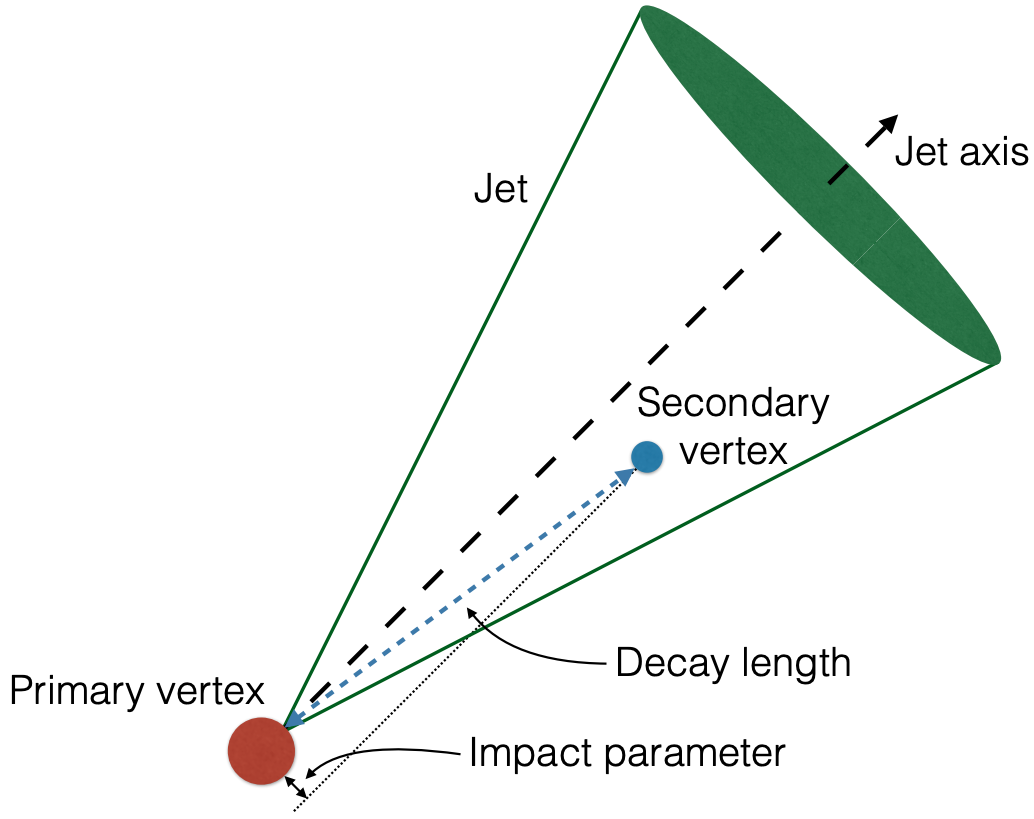
\includegraphics[width = 0.6\textwidth]{Chapter3/b_jet_production}
	 \caption{Illustration of the production of a \bjet with its characteristic 
	 second vertex~\cite{ATLAS:2019bwq}.} %Connelly:2017wlp
	\label{fig:Chap3:b_jet_production}
\end{figure}

The identification of \bjets involves a two-step process. Initially, low-level algorithms 
are employed to reconstruct the primary characteristics of the \bjets. Subsequently, 
the outcomes of these algorithms are combined in high-level algorithms that consist 
of multivariate classifiers. The various low-level algorithms can be categorised into 
three groups:

\begin{itemize}
	\item Impact-parameter-based algorithms:
	These algorithms employ the properties of individual tracks associated with a jet. 
	Tracks originating from $\Pbottom$-type hadron decay have distinct characteristics, 
	such as large impact parameters ($d_0$,$z_0$). Algorithms like IP2D and 
	IP3D~\cite{ATLAS:2017bcq} use the impact parameter significances of tracks within a
	jet to distinguish between \bjets and light-jets. Multivariate Analysis\footnote{MVA is 
	a statistical approach that analyses multiple variables together to identify patterns and 
	relationships in data. In this thesis, the MVA methods mentioned/used are the BDTs and NNs.}
	(MVA) methods are used by 
	other algorithms such as the RNN1P algorithm~\cite{ATLAS:2017gpy}, which exploits 
	spatial and kinematic correlations among tracks originating from the same B hadron
	 using a recurrent neural network\footnote{A neural network (NN) is a mathematical 
	machine learning model composed of interconnected artificial neurones that use activation 
	functions and weights to process input data, perform nonlinear transformations, and learn 
	from training examples through iterative adjustments of the weights to solve various tasks, 
	such as pattern recognition and regression. It performs similar tasks as those of the BDT 
	(see Appendix~\ref{chap:Appendix:BDT}).} (RNN).
	
	\item Secondary-vertex-based algorithms: 
	These type of algorithms use information from secondary vertices to create 
	discriminative variables for \btag. For instance, SV1~\cite{ATLAS:2017kle} is 
	a likelihood-based tagger that considers the invariant mass of particles in the
	secondary vertex, the ratio of track energies, the number of two-track vertices,
	and the $\Delta R$ separation between the primary-secondary vertex 
	and the jet direction.
	
	\item Decay-chain reconstruction: These algorithms aim to reconstruct the 
	complete decay chain of the B hadron. The JetFitter algorithm~\cite{ATLAS:2018nnq} is an example
	of this type. It uses the topology of weak \Pbottom- and \Pcharm-hadron decays 
	within the jet. It employs a Kalman filter~\cite{Fruhwirth:1987fm} to find a common line 
	connecting the primary, bottom, and charm vertices, enabling the reconstruction of 
	the  flight path of the B hadron and vertex positions.
\end{itemize}

High-level taggers, such as MV2 and DL1~\cite{ATLAS:2017bcq, ATLAS:2017gpy}, use the outcomes 
of low-level algorithms to determine the probability of a jet being classified as a 
\Pbottom-, \Pcharm-, or light-jet. MV2 employs a Boosted Decision Tree (BDT) architecture, while DL1 utilises 
a Deep Neural Network (NN). These high-level algorithms incorporate input from the IP3D, 
SV1, and JetFitter algorithms, along with the kinematic characteristics of the jets, 
including \pT and $\eta$. While MV2 is specifically trained to separate \bjets from
\Pcharm- and light-jet, the DL1 algorithm  provides a multidimensional output which
not only tags the \bjets but also the \Pcharm- and light-jets. 

One of the algorithms that composes the DL1 series is the \texttt{DL1r}~\cite{ATLAS:2017gpy}.
Its implementation as a multi-class NN architecture allows for a more compact 
memory usage compared to the previous BDT-based MV2c10 
algorithm~\cite{ATLAS:2019bwq}. The NN topology is comprised of fully connected 
hidden layers, and the hyperparameters are optimised to enhance the performance 
of \btag. The ultimate \texttt{DL1r} \btag discriminant is formulated as follows~\cite{ATL-PHYS-PUB-2017-013}:

\begin{equation}
\label{eq:Chap3:DL1r_discriminant}
	D_{\text{DL1r}}=ln \left(\frac{p_{b}}{f_{c} \cdot p_{c}+( 1 - f_{c})\cdot p_{ \text{light} }} \right)
\end{equation}

where $p_{b}$, $p_{c}$, $p_{\text{light}}$ and $f_{c}$ represent the \bjet,
\Pcharm-jet and light-flavour jet probabilities, and
the effective \Pcharm-jet fraction in the background training sample, respectively~\cite{ATLAS:2022qxm}. 
The \btagged jets are jets whose values of the \texttt{DL1r} are above a certain threshold, hereafter referred to as WPs. 
%Four WP are defined for the \texttt{DL1r}, the 
%70\% of the b-jets being selected in tt simulated event WP is used to define the b-jets.
%The efficiency of the \texttt{DL1r}, algorithm is measured in collision data
% In our analysis we use the DL1r tagger, it is described in \url{https://arxiv.org/pdf/2211.16345.pdf}
The efficiency of identifying \bjets~\cite{FTAG-2018-01} and the mis-tag rate of 
\ensuremath{c\text{-jets}}~\cite{ATLAS-CONF-2018-001} are measured using \ttbar event data. 
While the calibration of light-jets relies on events that involve a \PZ boson, 
following a procedure similar to the one described in Reference~\cite{ATLAS-CONF-2018-006}. 
The correction factors derived from these calibration analyses are subsequently applied to correct 
the simulated events. 
In Section~\ref{sec:ChaptH:ObjectDefReco:bjets} is discussed how the \texttt{DL1r} algorithm
is applied in this thesis.




%%
% top jets
%%
%\subsection{Top-quark-induced jets}
%\label{sec:Chap3:Reco:TopJets}
%There are various algorithms can distinguish jets originated from a top-quark decay 
%from those arising from gluons and all other quark flavours~\cite{ATL-PHYS-PUB-2020-017,ATLAS:2018wis}. 
%These techniques leverage characteristics of large-R jets produced by a top quark.
%\pablo{Nosotros no hablamos de top-induced jets. No tiene sentido hacer esto, no?}

%%%%%%%
%    MET    %
%%%%%%%
\section{Missing transverse energy}
\label{sec:Chap3:Reco:MET}
According to the principle of momentum conservation, the total sum of transverse 
momenta of all detected particles should be zero in the transverse plane. However, 
the presence of undetected particles can lead to an imbalance in this calculation, 
resulting in missing transverse momentum ($\overrightarrow{E}_{\text{T}}^{\text{miss}}$). 
%Although typically the module of this vector, \MET,  is what the physical analyses use.
This $\overrightarrow{E}_{\text{T}}^{\text{miss}}$ is typically associated with SM neutrinos, but it can also occur due 
to particles escaping the acceptance of the detector or being poorly reconstructed due to limitations in 
detector acceptance, finite detector resolution, detector inefficiencies presence of 
(temporary or permanent) dead regions, or any sources of noise.
% but it could also arise from 
%other weakly-interacting particles, including potential candidates for DM, which escape detection.

Therefore, the measurement of the magnitude of the missing transverse momentum (\MET) 
plays a crucial role in various analyses, such as the 
study of top-quark polarisation (see Section~\ref{sec:Chap1:Top:Polarisation}), which involves a 
final state with one neutrino (as in the search for the \tHq process presented in this work) or more neutrinos. 

The \MET is reconstructed by calculating the magnitude of the negative vector sum 
of the transverse momenta of all detected particles~\cite{ATLAS:2018txj, ATLAS:2018ghb}. 
This includes contributions from various particles such as leptons, photons, jets, and soft-event 
signals\footnote{Soft-event signals refer to reconstructed charged-particle tracks that 
are associated with the hard scattering vertex but not with any specific hard object.}.
%Since the \MET object is a composition of other physical objects with different \pT 
%resolutions, its calibration is non-trivial.



%%%%%%%
%    OLR    %
%%%%%%%
\section{Overlap removal}
\label{sec:Chap3:Reco:OverlapRemoval}
In ATLAS, the reconstruction of physics objects within the detector is primarily 
performed independently for each object. 
Ambiguity in the observed detector signatures can lead to the double-counting 
of signals, causing multiple physics objects to be defined simultaneously. This
is what is known as overlap. 
For instance, charged particle tracks in the inner tracking volume accompanied by 
energy deposits in the calorimeters could be interpreted as both an electron and a hadronic jet.
This ambiguity can arise from misidentification and duplication of objects or from 
the production of particles in close proximity (non-isolation), which may bias the 
reconstruction of one or both objects.

To address these reconstruction ambiguities, overlap removal is an essential step in 
all ATLAS analyses. In this analysis, the overlap removal is 
implemented based on the geometric proximity ($\Delta R$) between reconstructed 
objects. In Section~\ref{sec:ChaptH:ObjectDefReco:OverlapRemoval}, the
details of how this is done are provided.
 However, a recent advancement in the ATLAS core software introduced 
Global Particle Flow (GPF) links between jet constituents and physics objects that 
share a common detector element, such as a track or calorimeter cluster. These GPF links 
offer a cleaner approach for removing overlaps between jets and other physics objects. 
By explicitly examining shared detector signals among physics objects, it becomes possible to 
identify instances of double-counting of energy. If such overlaps are found, a set of criteria can 
be applied to determine which objects should be vetoed, ensuring accurate event reconstruction.








%Source: \url{https://indico.cern.ch/event/1131431/contributions/5059616/attachments/2512765/4319357/Ting_AIPabstract.pdf}


%POSTAMBLE
\begin{comment}
asdf
%\end{document}
%ENDPOSTAMBLE
\end{comment}
